\documentclass[prd, nofootinbib, floatfix, 11pt, tightenlines, times]{article}
\usepackage[paperwidth=8.5in,paperheight=11in,centering,margin=1.0in]{geometry}
\usepackage[pdftex]{graphicx}
\usepackage{natbib}
\usepackage[toc,page]{appendix}
\usepackage{subfig}
\usepackage{fancyvrb}
\usepackage{hyperref} 

% pdflatex S14report.tex; bibtex S14report; pdflatex S14report; pdflatex S14report; gv S14report.pdf

% Border around the figures
%\usepackage{float}
%\floatstyle{boxed}
%\restylefloat{figure}
\usepackage{framed}

\def\figdir{../figures}
\def\pasp{{\it PASP}}
\def\aap{{\it Astr.~Ap.}}     %Astronomy & Astrophysics%
\def\aaps{{\it A\&AS}}
\def\apj{{\it ApJ}}
\def\A{{\tt A}}
\def\B{{\tt B}}
\def\C{{\tt C}}
\def\D{{\tt D}}
\def\E{{\tt E}}
\def\P{{\tt P}}

\title{\vspace{-22mm} \Large{Report on Summer 2014 Production: Analysis of DCR\vspace{-10mm}}}
\date{\today}
\author{
%  Andrew Becker, Simon Krughoff, Andrew Connolloy {\it for LSST Data Management}
}
\begin{document}
\maketitle\vspace{-8mm}

The goals of this Summer 2014 (S14) task were to understand the scope
of the differential chromatic refraction (DCR) issue using a realistic
range of stellar spectral energy distributions (SEDs).  We used LSST
catSim's all--sky catalog of stellar sources, including their number
counts and magnitude distributions, to estimate how many sources will
be detected at 5--sigma in the LSST $ugri$--bands.  The SED of each of
these sources was used to model the per--passband refraction, and then
the differential refraction with respect to a single reference SED, as
a function of airmass.

We first examined the amplitude of the vector connecting the DCR of a
source from 2 different observations.  The DCR in a single observation
was calculated with respect to the reference SED.  We assume that
objects having this reference SED may be used to define an astrometric
reference frame, within which the red/blue stars will move based upon
the effects of DCR.  A differential DCR vector may then be defined
through comparison with the amplitude and orientation of DCR in a
second observation, which should represent the shape of a dipole
arising in image subtraction from images taken under these two
conditions, assuming that astrometric registration proceeds using
objects the color of the reference SED.

We placed our reference SED at airmass 1.25 to provide a DCR ``zero
point''.  We then varied the airmass and parallactic angle of a second
observation, and calculated the amplitude of the differential DCR
vector for each of 6292 SEDs.  This amplitude is band, airmass, and
parallactic angle dependent.  We quantified the $ugriz$--band
dependence of this vector on airmass and parallactic angle difference:
nearly all stars in the $g$--band, and $r$--band sources with
parallactic angle differences of 20 degrees or airmass differences of
0.15, will exhibit differential DCR amplitudes larger than 5mas.  In
the $i$--band, this is relaxed to parallactic angle differences of 25
degrees or airmass differences of 0.2, with the majority of $i$--band
sources exhibiting DCR coming from the M--dwarf population.  In the
$z$--band only large differences in parallactic angle yield
significant numbers of objects with this vector amplitude larger than
5mas.

We then examined the degree to which DCR amplitudes can be modeled
using broad--band color and airmass terms.  It is presumed a process
like this must be established to undo or mimic the effects of
refraction when coadding or subtracting data.  We additionally looked
at how errors in source colors impacted these model estimates of DCR.
A random forest regression model using source colors, airmass terms,
and color--airmass cross terms was found to provide the best model of
both refraction and DCR vs. airmass, judged using a cross--validation
sample of data not used in the model fitting.  We found that $u$--band
refraction and DCR models may be built that have RMS residuals of less
than 5mas at all zenith distances, but having a tail where 1\% of
sources show model residuals larger than 5mas beyond 20 degrees zenith
distance.  Errors in source color further degrade this, such that 10\%
misestimates of source color yield 5mas model residuals for 1\% of
stars at 5 degrees zenith distance.  These results worsen at larger
zenith distance.  In the $g$--band, both refraction and DCR may be
modeled to zenith distance of 50 degrees, such that $10^{-5}$ of stars
or less show residuals of 5mas.  Photometric errors of $\sim 2.5\%$ or
greater significantly degrade our ability to model $g$--band
refraction and DCR.  In the $riz$--bands, the fraction of stars
exhibiting larger than 5mas residuals from the model are at the
$10^{-5}$ level or lower.

To summarize, predicting the amplitude of DCR in the $u$--band will be
a significant difficulty under nearly all realistic conditions.  DCR
in the $g$--band appears to be largely (but not entirely) approachable
using non--linear regression models and color/airmass terms.  DCR in
the $riz$--bands may be modeled with small residuals using the same
class of regressions.  We note that these results are restricted to
the stellar SEDs studied in this report.  This research does not
address the actual methods needed to compensate for the DCR
predictions coming out of this modeling process, although we provide
some thoughts on possible techniques within the report.

\clearpage
\tableofcontents
\clearpage

\section{Scope and Goals}

The goal of this research was to model the frequency at which
DCR--related dipoles will arise in LSST data.  This includes the
frequency of dipoles in the absence of any modeling, and after
attempts to predict and compensate for the effect.  Implementation of
actual methods to compensate for total and differential refraction at
the pixel level were left as stretch goals that were preempted by the
LSST 2014 documentation sprint.

We used the theoretical and simulation studies undertaken in Winter
2014\footnote{https://dev.lsstcorp.org/cgit/contrib/W14/ImageDifferencing.git/tree/report/W14report\_current.pdf}
to understand the amplitude of astrometric offsets that lead to
measurable dipoles in high S/N point sources: there is 1\% chance of
generating a measurable dipole when there are unmodeled astrometric
residuals of $\sim$5 mas in 0.6'' seeing, or $\sim$7 mas in 0.88''
seeing.  To create a realistic all--sky 5--sigma sample of potential
DCR sources, we used the actual SED population and brightness
distribution of {\it all} objects from the catalogs used to seed the
LSST image simulations.  The SED of each source was used to find exact
per--source and per--passband refraction amplitudes, as a function of
airmass.  The broad--band colors were then used as inputs to a
modeling effort to understand our ability to predict refraction as a
function of source color and airmass.  We trained multiple regression
models on 2/3 of these data, with color and airmass terms as features,
and with the SED--derived total or differential refractions as the
values we intended to predict.  The other 1/3 of these data were used
to assess the predictive power of these models.

All tasks were undertaken under epic DM-246, ``Investigate
compensation for Dcr''.  The main stories were:

\begin{itemize} 

\item {\bf DM-787}: Using a realistic distribution of all SEDs from
  catSim, understand the bulk numbers of stars that we expect to
  exhibit DCR above a fiducial amplitude of 5mas.

\item {\bf DM-788}: With this same distribution of catSim sources, use
  their spectral energy distributions to understand the per--source
  refraction amplitudes.

\item {\bf DM-789}: Model and predict the per--source refraction
  amplitudes using only broad--band color and airmass terms.  This
  includes linear regression and non--linear machine learning
  techniques.  Understand how well the source color must be measured
  to be able to predict the refractive astrometric shift to within in
  a given tolerance of 5mas.

\item {\bf DM-790}: With this same distribution of catSim sources, use
  their spectral energy distributions to understand the per--source
  differential chromatic refraction (DCR) amplitudes.

\item {\bf DM-791}: Model and predict the per--source DCR using only
  broad--band color and airmass terms.  Understand how well the source
  color must be measured to be able to predict the DCR astrometric
  shift to within in a given tolerance of 5mas.

\end{itemize} 

\section{Results}

\subsection{\bf DM-787}

The first task was to understand the magnitude of the problem: how
many total stars do we expect to exhibit the effects of differential
chromatic refraction at an amplitude of 5mas.  As inputs, we used the
entirety of the catalog simulation suite of SEDs.  For each discrete
SED, the numbers of stars in the catalog were extracted from the
catSim database, in 1--magnitude bins in apparent $g$--band magnitude.
Their SEDs were used to calculate magnitudes in the $uriz$ passbands,
which were used to calculate the total numbers of objects brighter
than fiducial 5--sigma limiting $ugriz$ magnitudes of $[23.9, 25,
  24.7, 24, 23.3]$, respectively.  This resulted in the numbers of
sources of a given SED, per passband, that LSST is expected to detect
above 5--sigma.

Using the flux vs. wavelength profile of each SED, and the
transmission profiles of the LSST $ugriz$ passbands, we were able to
calculate a flux--weighted refraction offset for each source, within
each passband, and for a given airmass.  This offset is assumed to be
the ``truth'' in the analyses that follow.

We chose a reference SED with median g-r colors ({\tt
  km15\_5250.fits\_g05\_5470.gz}) to calculate DCR against.  We first
calculated the amplitude of refraction for this reference source at an
airmass of 1.25, and also did so for each of the other 6292 SEDs in
the catSim database.  The DCR amplitude for each source is trivially
calculated as the difference of the reference and source refraction
amplitudes.  We then calculated both the amplitude and direction of
DCR in a {\it second} observation, with a range of differing airmasses
and/or parallactic angles.  This difference in DCR vector is what will
manifest as a dipole in a subtracted image (e.g. if all images are
taken under the same airmass and parallactic angle conditions, DCR
will be the exact same in all images, and there will be no dipoles due
to this effect).  The total fraction of sources that exhibited a
differential DCR amplitude greater than 5mas was used to color code
the $\Delta$~airmass and $\Delta$~parallactic angle grid in
Figure~\ref{fig:dcr}, for each of the $griz$ passbands.  The {\it red}
line shows where the fraction of sources exhibiting DCR larger than
5mas is larger than 1\% (i.e. 1\% of stars have a 1\% chance of
yielding DCR dipoles in a difference image).  We note that in the
$g$--band 1\% of all sources will exhibit differential DCR larger than
5mas for even small differences in airmass and parallactic angle
between 2 images, for a reference airmass of 1.25.  In the $r$--band a
difference of 20 degrees of parallactic angle at the same airmass, or
a difference of 0.15 in airmass, will yield an enhanced DCR dipole
rate.  In $i$--band this is relaxed to $\Delta$~airmass of 25 degrees
and $\Delta$~angle of 0.2.  By $z$--band only large differences in
parallactic angle yield an enhanced rate of dipoles.

To understand how much of the DCR dipole signal comes from the
majority population of red M--dwarfs, we repeated this analysis but
ignoring the M--dwarf SEDs.  These results are plotted in
Figure~\ref{fig:dcrnoM}.  By comparing these results with those in
Figure~\ref{fig:dcr}, we see that much of the DCR sensitivity in the
$i$--band comes from these M--dwarfs.  However, in the bluer bands,
LSST will still be primarily sensitive to DCR from the other
populations of objects, given the intrinsic faintness of M--dwarfs in
these bands.

\begin{figure}[!t]
  \centering
  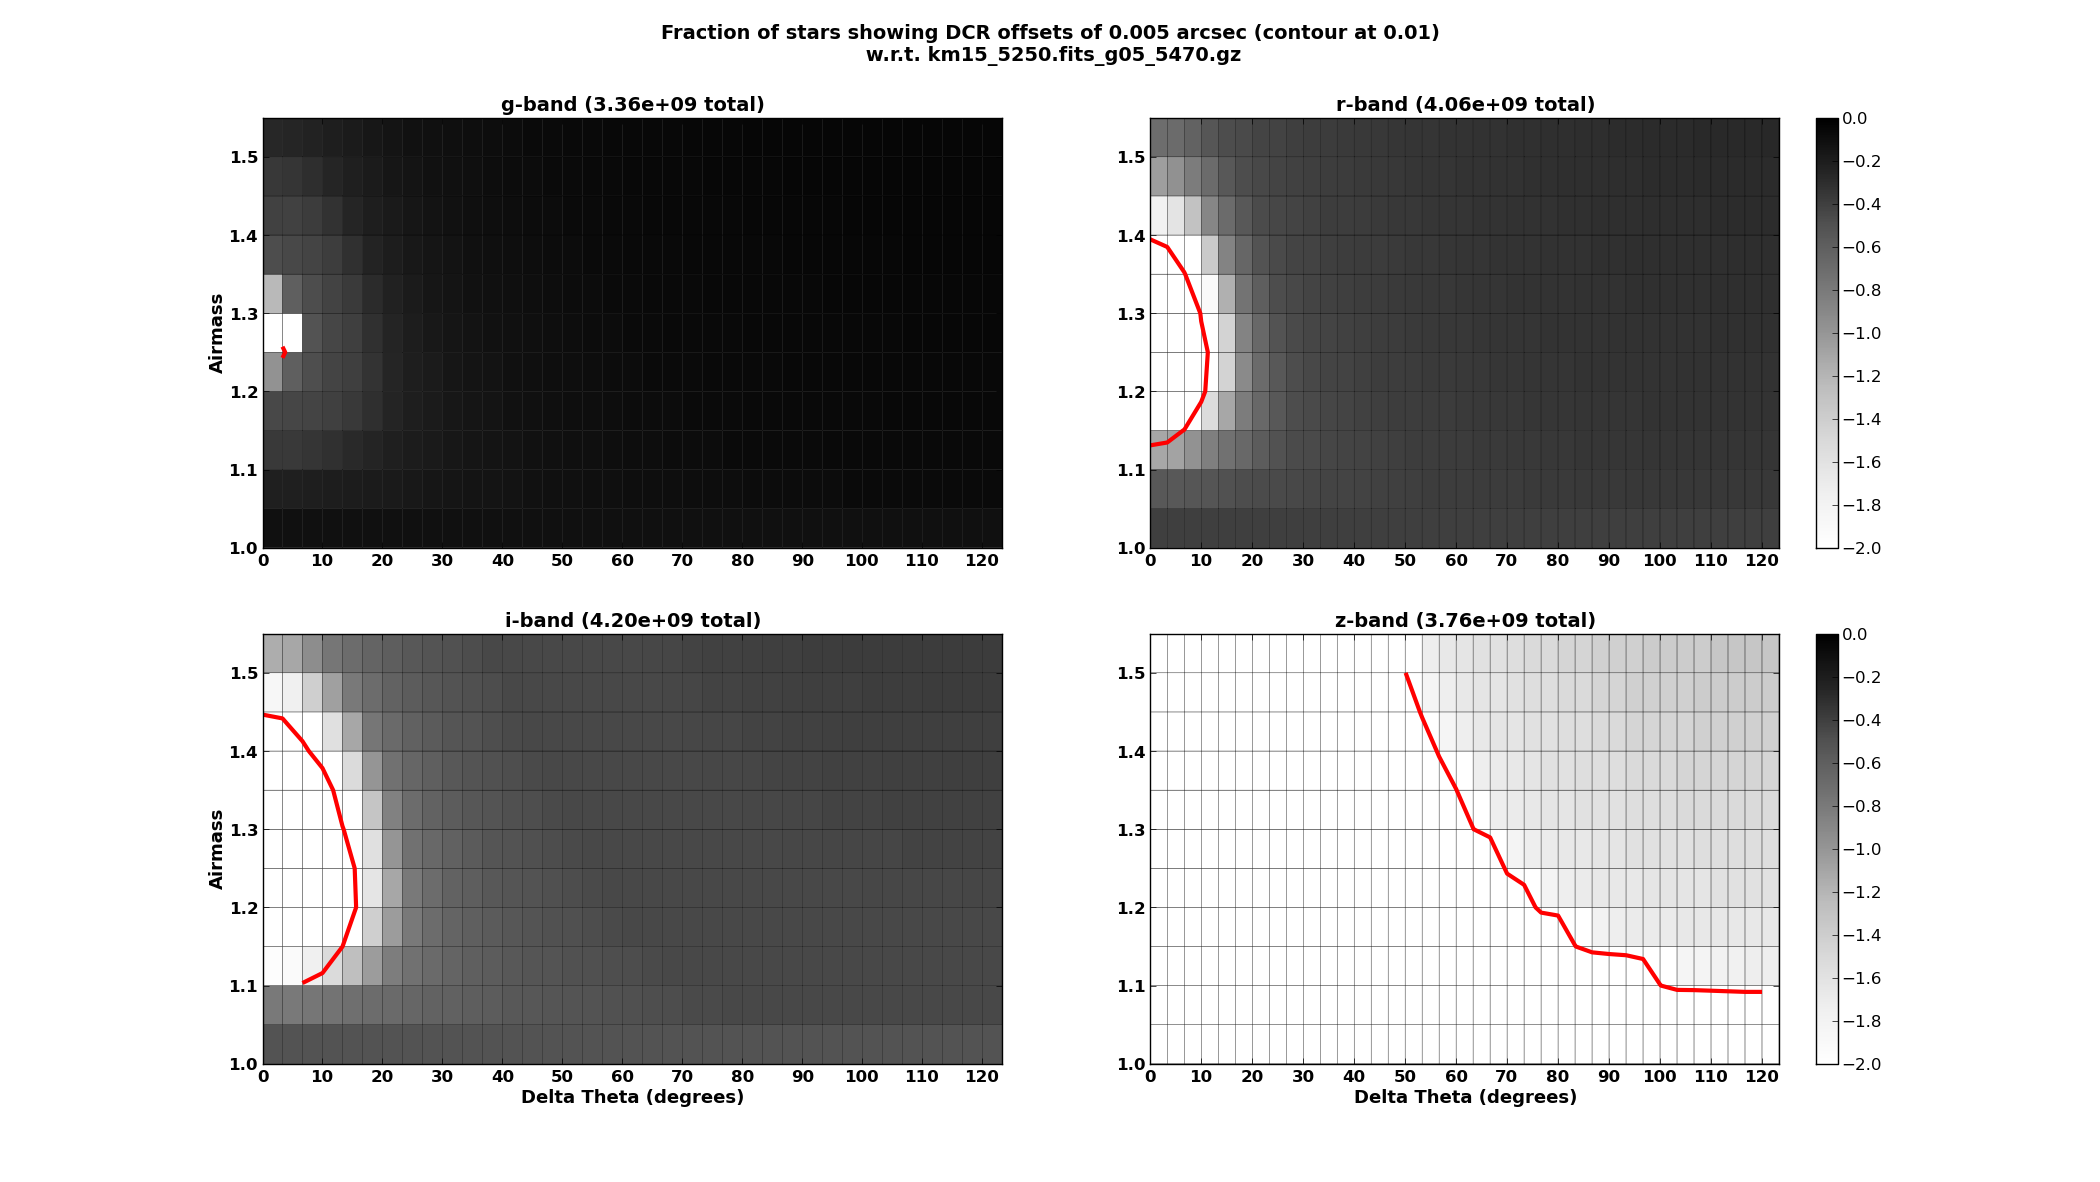
\includegraphics[width=1.1\textwidth]{\figdir/calculateSedDcr2.png}
  \caption{{\bf Fraction of Stars Exhibiting DCR Offsets Larger than
      5mas}: We plot the fraction of {\it all} stars in the catSim
    database, brighter than 5--sigma, that will have differential DCR
    amplitudes larger than 5mas compared to reference SED {\tt
      km15\_5250.fits\_g05\_5470.gz} at airmass 1.25.  The
    per--passband total numbers of stars brighter than 5--sigma are
    listed in the title of each subpanel.  Each subpanel shows
    heatmaps with the log10 fraction of these stars having DCR
    amplitudes larger than 5mas, for differences in airmass and
    parallactic angle, for stars in the $griz$--bands.  This figure
    may be recreated using the script {\tt
      python/calculateSedDcr2.py}.}
  \label{fig:dcr}
\end{figure}

\begin{figure}[!t]
  \centering
  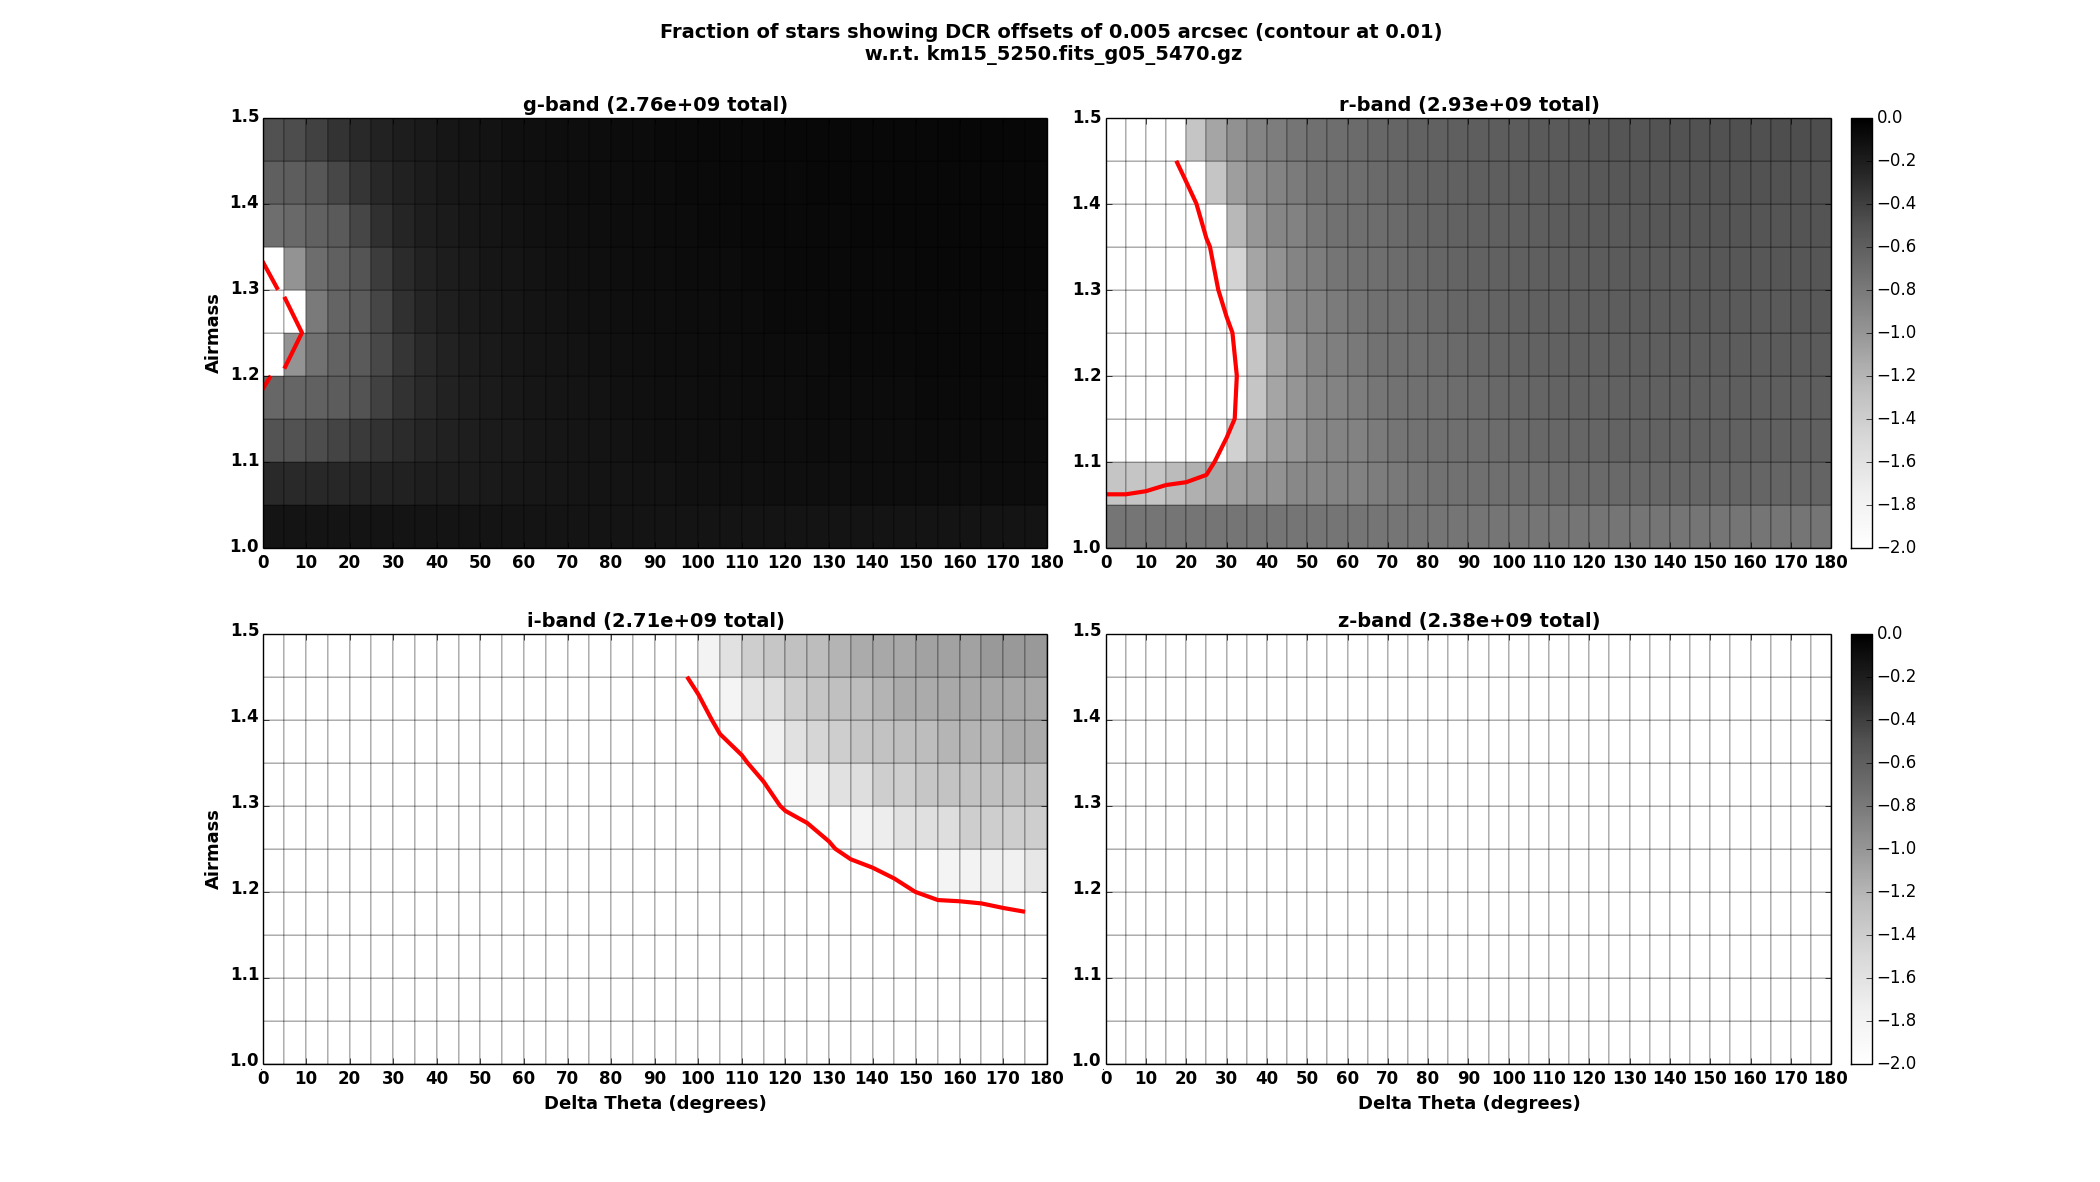
\includegraphics[width=1.1\textwidth]{\figdir/calculateSedDcr2M.png}
  \caption{{\bf Fraction of non--M Dwarf Stars Exhibiting DCR Offsets
      Larger than 5mas}: Same as Figure~\ref{fig:dcr}, but {\it
      excluding} the majority M-dwarf population of objects.}
  \label{fig:dcrnoM}
\end{figure}

\subsection{\bf Modeling Refraction: DM-788 and DM-789}

In this work we assessed the extent to which we can predict the amount
of refraction from broadband colors and airmass terms.  In addition,
we also determined the level of precision at which we need to measure
these colors before our estimate of refraction is significantly
impacted.  We defined ``significant'' as yielding a difference of 5mas
w.r.t. the ``true'' amount of refraction determined using SEDs.

The first step in this process was to calculate the per--SED,
per--passband refraction amplitudes as a function of airmass, as
described above.  This reflects the underlying ``truth'', in terms of
refraction amplitude, that we attempted to model.  For each source, we
calculated the set of broadband colors $u-g$, $u-r$, ..., $i-z$ to
provide a coarse estimate of the underlying SED.  It is assumed that
LSST will have some measured estimate of these values available for
each source, but no additional information regarding the true SED.  At
a range of airmasses, we calculated airmass terms $tan(z)$ and
$tan^3(z)$ where $z$ is the zenith distance of the observation
\citep[e.g.][]{1996PASP..108.1051S}.  We defined a refraction model
using these terms, in order to predict the amplitude of refraction as
a function of source color and airmass:
\begin{eqnarray}
  R(SED;z) & = & \sum_{i={\it ugriz}}\sum_{j>i} A_{ij} (m_i - m_j)        \\ \nonumber
  & + & \sum_{i={\it ugriz}}\sum_{j>i} B_{ij} (m_i - m_j) \times tan(z)   \\ \nonumber
  & + & \sum_{i={\it ugriz}}\sum_{j>i} C_{ij} (m_i - m_j) \times tan^3(z) \\ \nonumber
  & + & D \times tan(z) + E \times tan^3(z).                              \\ \nonumber
\end{eqnarray}
and explored several ways to solve for $[A_{ij},B_{ij},C_{ij},D,E]$.
It is assumed that the parallactic angle, and thus the direction of
refraction, is known.

A linear regression was performed using the following methodology:
\begin{Verbatim}[frame=single]
import numpy as np  
A = np.array((nsed * nairmass, nterms))
R = np.array((nsed * nairmass,))
# Fill array A with features; fill array R with SED-based refractions
cov = np.linalg.inv(np.dot(A.T, A))
soln = np.dot(cov, np.dot(A.T, R))
pred = np.dot(soln, A.T).
\end{Verbatim}
Here {\tt nsed} is the number of discrete SEDs in the database (6293),
{\tt nairmass} are the airmasses to evaluate the model at (0..49
degrees in steps of one degree), and {\tt nterms} are the total number
of features in the model.  The mean and root--mean--square residuals
of the prediction {\tt pred} were used to ascertain the goodness of
fit.  We found that this linear model was insufficient to describe the
effects of refraction.

Accordingly, we further explored non--linear regressions using the
scikit--learn classes {\bf LinearRegression} (effectively the same as
above), {\bf ExtraTreeRegressor}, {\bf DecisionTreeRegressor}, and
{\bf RandomForestRegressor}.  We used 2/3 of the inputs to fit the
regression, and validated the predictive power of each model using the
other 1/3 of the data.  In most cases we found that the random forests
provided the best results, in terms of the mean model residuals as a
function of airmass, the RMS residuals as a function of airmass, and
the fraction of stars showing unmodeled residuals larger than 5mas.
We summarize these results for $u$--band in Figure~\ref{rmodel}, with
$griz$--band data found in Figure~\ref{rmodel2} in
Appendix~\ref{appx:rmodel}.  Within each subfigure, we plot the mean
({\it top}) and RMS residuals ({\it middle}) of the cross--validation
sample, along with the fraction of all cross--validation stars that
are misfit by more than 5mas ({\it bottom}).

\begin{figure}[!t]
    \centering
    \subfloat[$u$--band]{{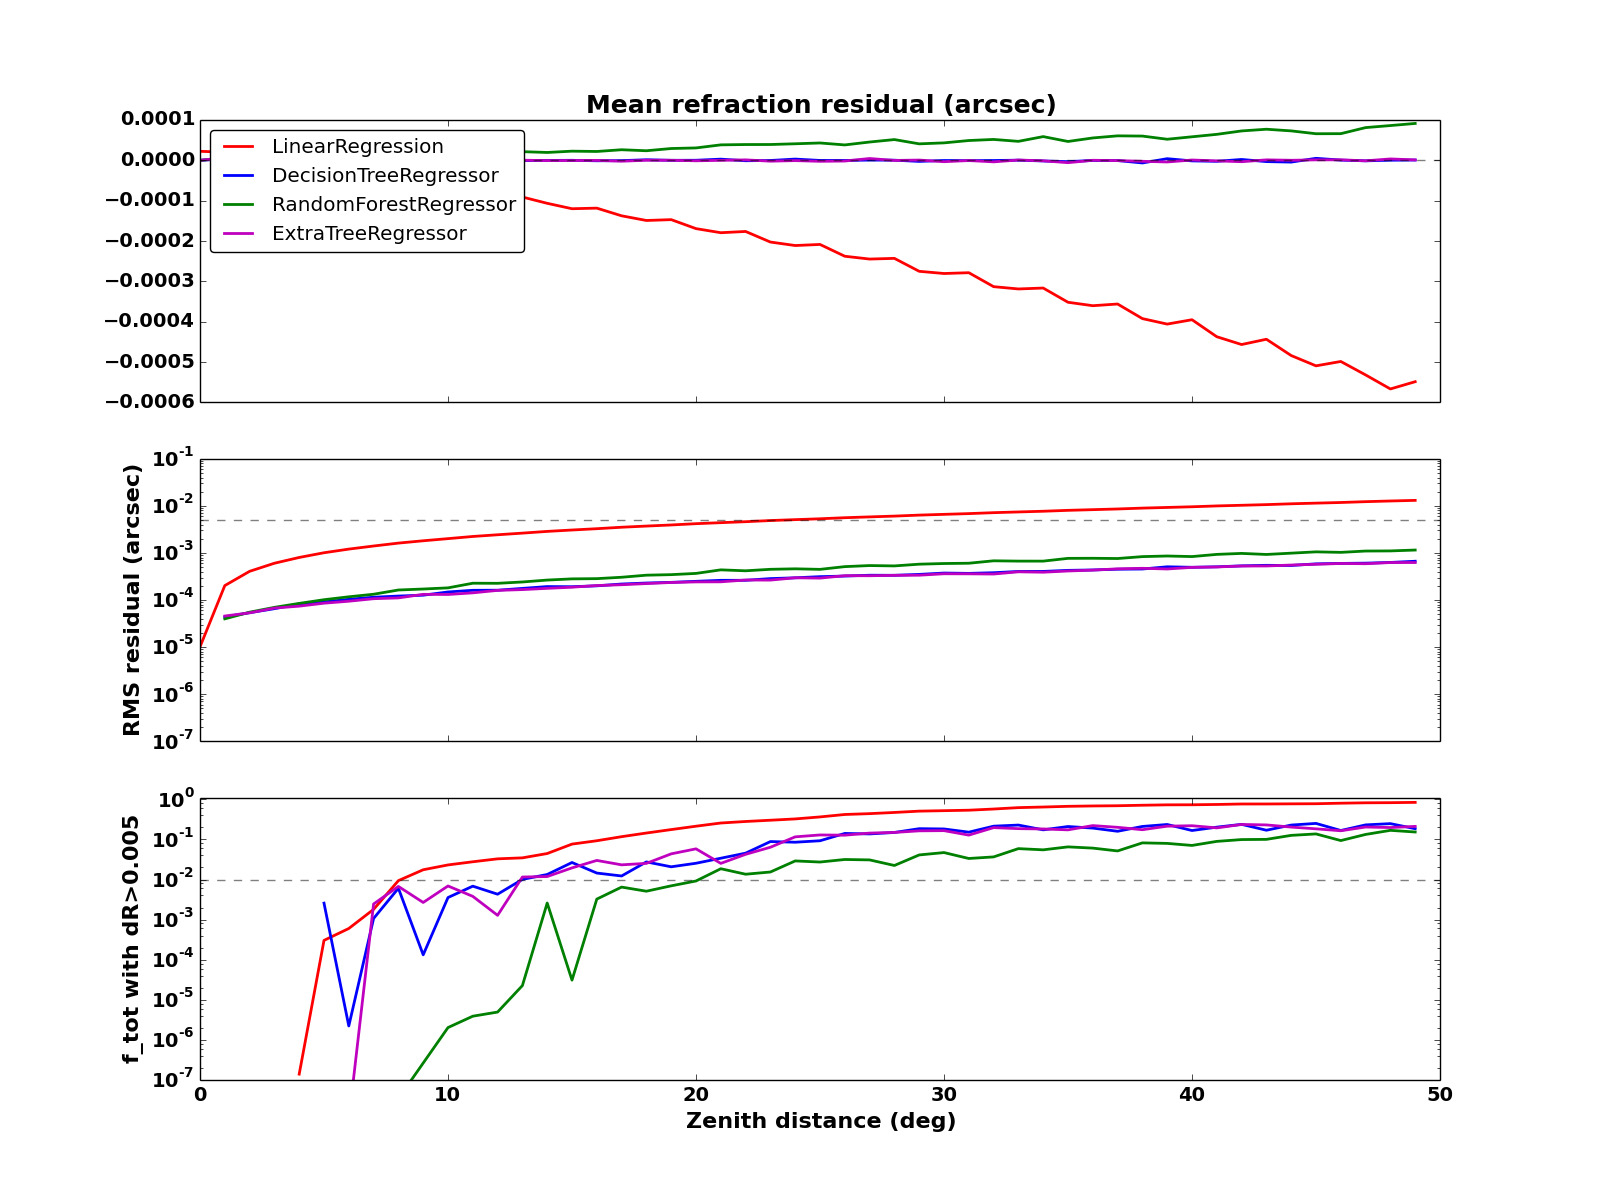
\includegraphics[width=\textwidth]{\figdir/R_u_A.png} }}
    \caption{{\bf Modeling Refraction Using Broadband Colors}: This
      figure summarizes the quality of the $u$--band regressions for
      the modeling of refraction as a function of airmass.  We used
      2/3 of the catSim SEDs to train the model, and 1/3 of the data
      to test the predictive power of the model.  This figure shows
      the mean residuals ({\it top}) of the out--of--sample data, the
      root--mean--square residuals ({\it middle}), and the fraction of
      the out--of--sample sources with residuals larger than 5mas
      ({\it bottom}).  We plot curves for each of the {\bf
        LinearRegression}, {\bf ExtraTreeRegressor}, {\bf
        DecisionTreeRegressor}, and {\bf RandomForestRegressor}
      models.  We find that the linear regression provides a biased
      estimate of refraction at all airmasses, as does the random
      forest model, to a lesser degree.  The RMS residuals of the
      $u$--band models are less than 5mas at all airmasses.  However,
      there is a tail of objects that exhibit 5mas residuals beyond
      approximately 20 degrees zenith distance (the horizontal line in
      the bottom panel indicates where 1\% of the objects show
      residuals larger than 5mas).  The random forest model provides
      the best model in terms of minimizing the number of these
      outliers.  Similar plots for the $griz$--bands can be found in
      Figure~\ref{rmodel2}.  This figure was created using the script
      {\tt python/calculateSedDcr3ML.py}.}
    \label{rmodel}
\end{figure}

Several trends are apparent.  First, the linear regression model is
too inflexible to provide an unbiased model of refraction as a
function of airmass.  Second, the random forest regression generally
provides an unbiased fit and the smallest RMS residuals as a function
of airmass, with a notable exception being in the $u$--band, where the
extra tree and decision tree regressors outperform.  Finally, the
refraction model is such that less than 1\% of all stars in the
database will have residuals larger than 5mas out to 20 degrees zenith
distance in the $u$--band, using the random forest model, which yields
the smallest fraction of these outliers.  In all other passbands, and
at all airmasses, the fraction of stars with large unmodeled residuals
is orders of magnitude smaller.  We note that the random forest model
is significantly better than all other models in these bands
(Figure~\ref{rmodel2}).  The ``spikes'' in these residuals plots come
from a small number (typically less than 3) of discrete SEDs that
comprise a fractionally large portion of the out--of--sample data.

For the random forest model we retained the feature importance
metrics.  We found for all refraction models, the $tan(z)$ and
$tan^3(z)$ terms primarily drove the model, followed by three color
and color--airmass interaction terms at nearly equal importance: in
the $u-g; g-r; g-i; r-z; u-i$ colors for the $ugriz$ bands,
respectively.  For example, for the $u$--band, the top 5 terms were
$tan(z)$, $tan^3(z)$, $u-g$, $(u-g) \cdot tan(z)$, $(u-g) \cdot
tan^3(z)$.  A figure showing the relative feature importance for
modeling refraction in the $u$--band is shown in
Figure~\ref{fig:feat}.

\begin{figure}[!t]
  \centering
  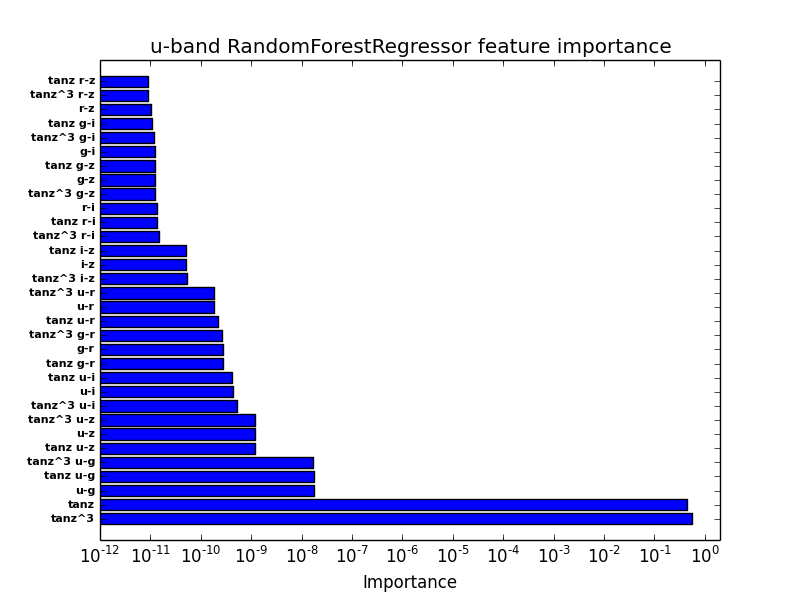
\includegraphics[width=1.1\textwidth]{\figdir/R_u_A_50_rfr.png}
  \caption{{\bf Feature Importance}: This figure shows the relative
    importance of features used to model refraction in $u$--band using
    a random forest regression.}
  \label{fig:feat}
\end{figure}


We note that we did {\it not} attempt to optimize hyperparameters of
the models (e.g. the number of trees in the random forest).  We did
explore weighted regressions, where each point in the training
contributed proportional to the number of SEDs in the database, but
this did not significantly alter the model's predictive ability.
Because of the random nature of some of these models, we did notice
subtle differences (e.g. in feature importance) in the results between
different runs.

\subsubsection{\bf Required Photometric Precision \label{sec:rcolor}}

In order to understand LSST's ability to model refraction, as a
function of uncertainty on source color, we repeated the above
analysis but including a random offset to the colors of the
cross--validation test data.  These offsets were intended to mimic the
effects of measurement uncertainty on the source color.  Offsets were
drawn from normal distributions with means of zero (no bias) and
widths of (0.01, 0.025, 0.05, 0.075, 0.1) magnitudes in color.  These
were added to the SED--derived broadband colors and the regression
model evaluated to generate a ``noisy'' prediction.  We only used the
{\bf RandomForestRegressor} since this model seemed to perform best
under most conditions.  Results are summarized in Figure~\ref{rerr}
for $u$--band, and Figure~\ref{rerr2} for $griz$--bands.

We find that in the $u$--band, even 1\% photometric scatter provides a
significant degradation in the modeling of refraction, with 1\% of
objects having residuals larger than 5mas beyond 10 degrees zenith
distance, compared to a similar limit of 20 degrees when there are no
photometric errors.  At 10\% photometric error in color, modeling
refraction beyond 5 degrees zenith angle becomes difficult.  Looking
at the bluer passbands (Figure~\ref{rerr2}), 2.5\% photometric error
is sufficient to degrade the models predictive power in $g$--band
beyond 40 degrees, and 5\% error degrades the model beyond 25 degrees.
In the $r$--band and beyond, the model is sufficient to predict
refraction with even 10\% photometric errors in source color, out to
50 degrees zenith distance.  However, there will be a small population
of outliers ($\sim 10^{-4}$) at large zenith distances that will show
$r$--band refraction errors larger than 5mas.  Given the large numbers
of stars expected to be detected ($\sim 3e9$), this translates to
approximately one object per sensor having a 1\% chance of yielding a
dipole, in $r$--band, at 50 degrees zenith distance ($3e9 \times 1e-4 /
2000$ LSST fields).

\begin{figure}[!t]
    \centering
    \subfloat[$u$--band]{{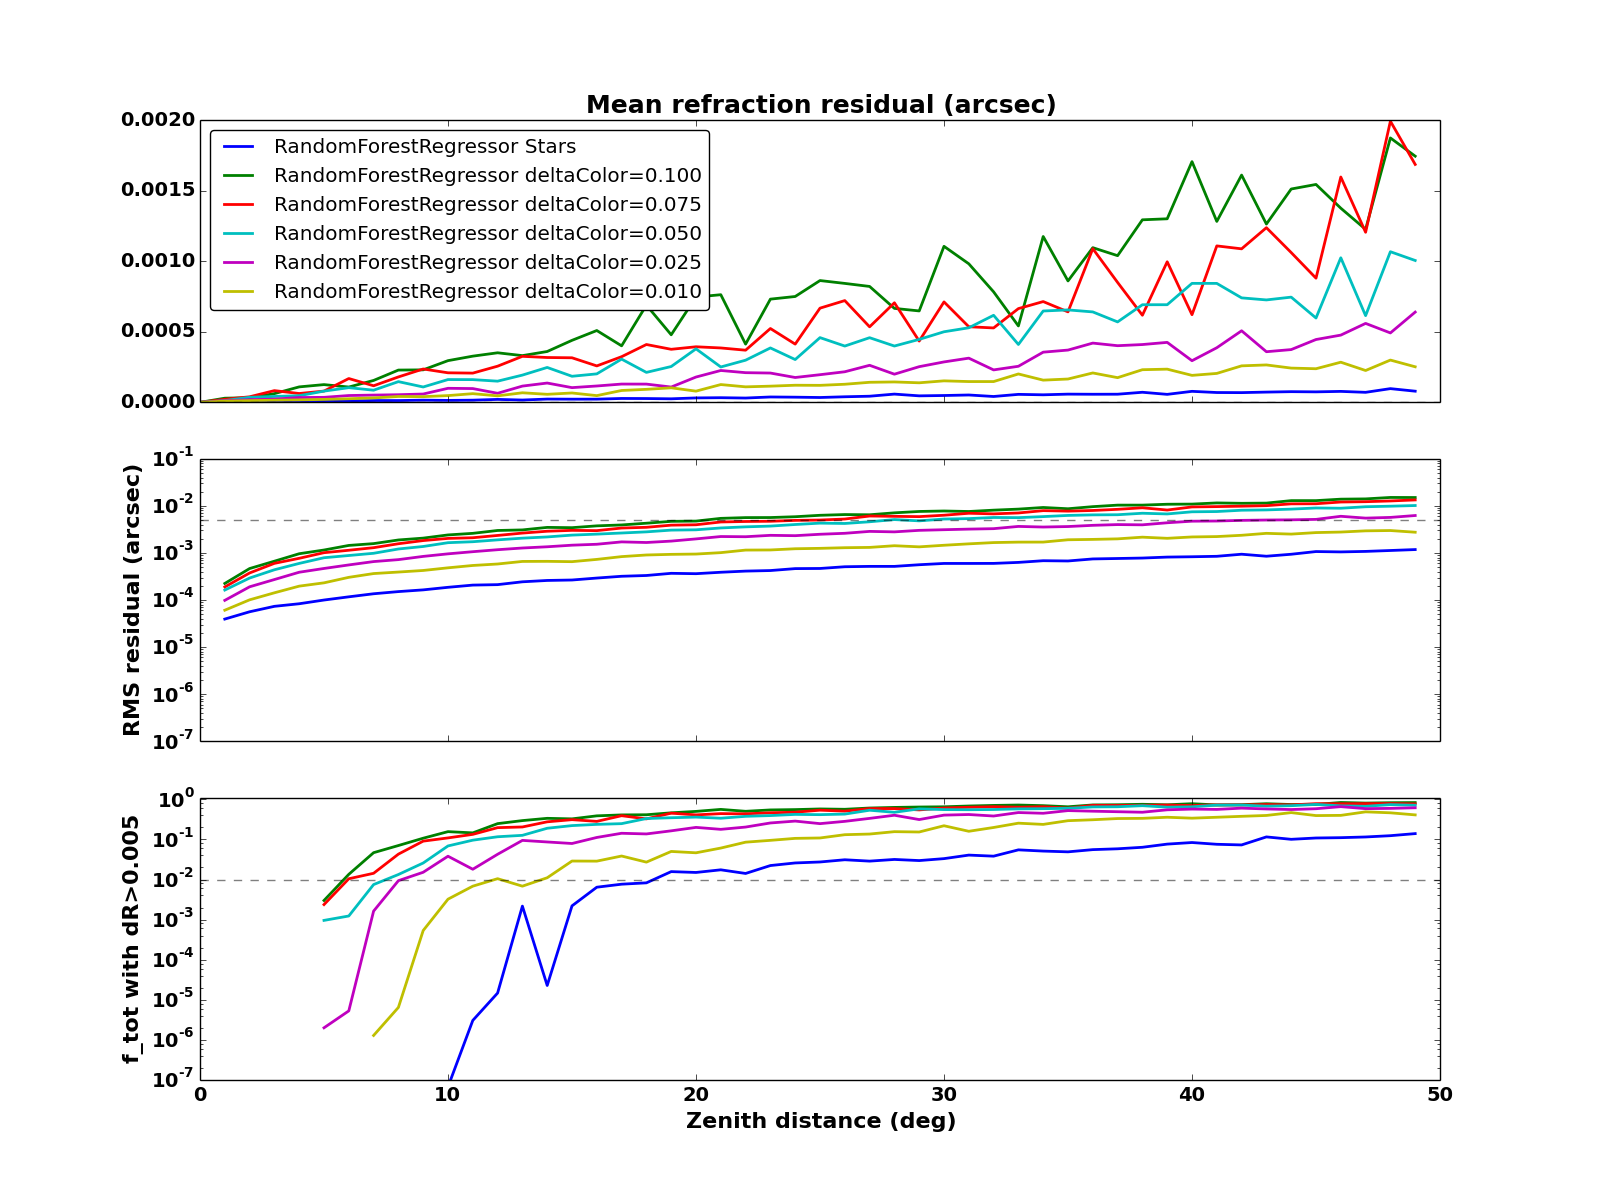
\includegraphics[width=\textwidth]{\figdir/R_u_deriv.png} }}
    \caption{{\bf Mapping Color Errors to Refraction Misestimates}: 
      This figure shows the results of evaluating a noisy dataset
      using a $u$--band {\bf RandomForestRegressor} regression model
      on refraction amplitude.  The {\it top} panel provides a measure
      of the mean model offset as a function of airmass, the {\it
        middle} panel the RMS offset, and the {\it bottom} panel the
      fraction of outliers with offsets larger than 5mas.  An
      out--of--bag sample comprising 1/3 of the SED dataset was used
      to evaluate these models.  In {\it blue}, we show the core model
      performance in the absence of photometric errors.  The other
      lines show the degradation of the model when the test data have
      random offsets of 1\% to 10\%.  Similar plots for the
      $griz$--bands can be found in Figure~\ref{rerr2}.  This figure
      was created using the script {\tt
        python/calculateSedDcr3ML\_deriv.py}.}
    \label{rerr}
\end{figure}

\subsection{\bf Modeling DCR: DM-790 and DM-791}

In this work we determined the extent to which we can predict the
amount of {\it DCR} from the broadband colors and airmass terms,
similar to the analysis above.  We came to similar conclusions from
the training process, in that the random forest regression yields the
model with the most predictive power (with the exception of the
$u$--band) and fewest outliers (in all bands).  We also reached very
similar conclusions on the degree to which DCR is model--able, given
broad--band colors and airmass (Figure~\ref{dcrmodel} for $u$--band,
and Figure~\ref{dcrmodel2} for $gri$--band).

\begin{figure}[!t]
    \centering
    \subfloat[$u$--band]{{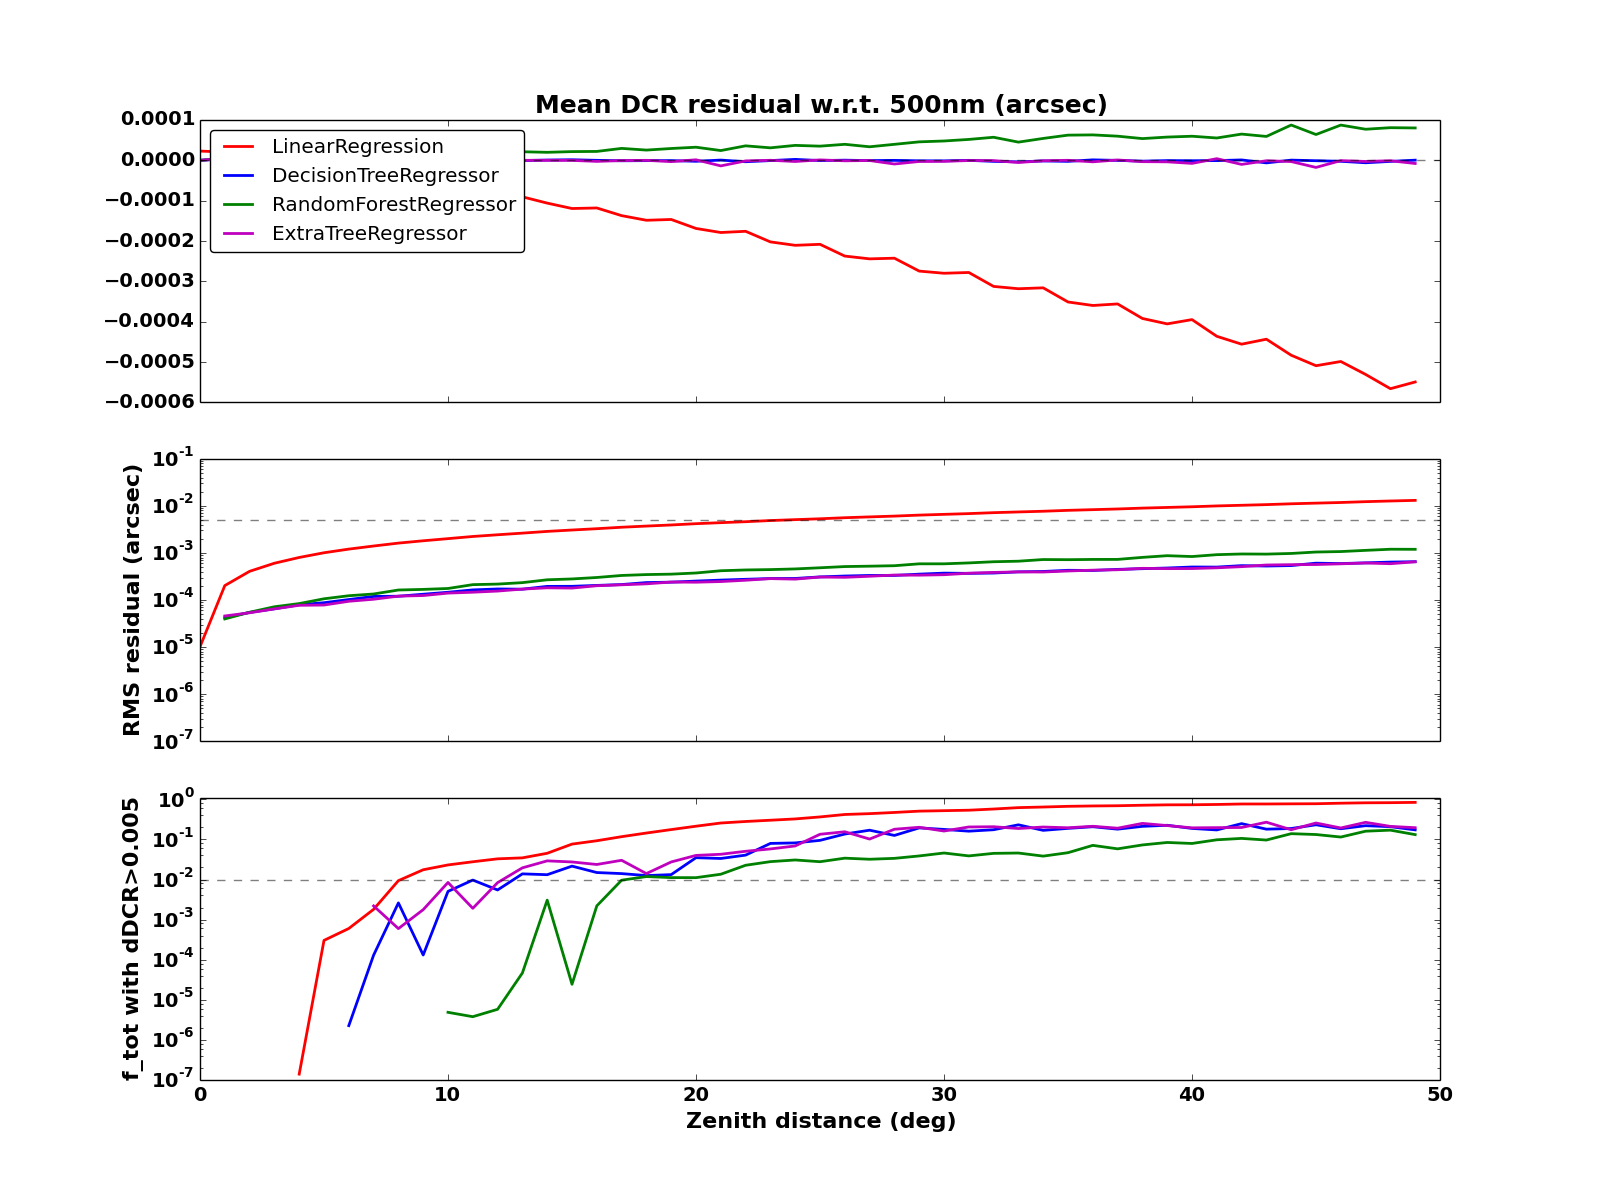
\includegraphics[width=\textwidth]{\figdir/DCR_u_A.png} }}
    \caption{{\bf Modeling DCR Using Broadband Colors}: Similar to
      Figure~\ref{rmodel}, but for a regression model that predicts
      DCR instead of refraction.  Similar plots for the $griz$--bands
      can be found in Figure~\ref{dcrmodel2}.  This figure was created
      using the script {\tt python/calculateSedDcr4ML.py}.}
    \label{dcrmodel}
\end{figure}

We found that DCR in $u$--band was predictable out to a threshold of
20 degrees zenith distance, beyond which 1\% of stars deviated from
the model by more than 5mas.  In the $g$--band and beyond
(Figure~\ref{dcrmodel2}) there were a small fraction of sources (of
order $10^{-6}$) exhibiting residuals larger than 5mas beyond zenith
distance of 40 degrees, which translate to approximately 1 per LSST
field.

\subsubsection{\bf Required Photometric Precision}

In order to understand LSST's ability to model DCR, as a function of
uncertainty on source color, we repeated the above analysis including
a random offset to the colors of the cross--validation test data.
This analysis was performed similar to the refraction analysis in
Section~\ref{sec:rcolor}.  Results are summarized in
Figure~\ref{dcrerr} for $u$--band, and Figure~\ref{dcrerr2} for
$gri$--bands.

We find similar results to the refraction analysis.  In the $u$--band,
DCR estimates for objects having photometric errors of 10\% will be
inexact beyond zenith distances of 5 degrees (Figure~\ref{dcrerr}).
In the $g$--band, 1\% photometric errors are sufficient to avoid
significantly wrong DCR predictions, but with 2.5\% photometric
errors, 1\% of stars at 35 degrees zenith distance will have their DCR
amplitudes misestimated by more than 5mas (Figure~\ref{dcrerr2}).  In
the $r$--band, there is a small population of objects beyond zenith
distance of 40 degrees (approximately 1 per sensor) that will exhibit
model residuals larger than 5mas when photometric errors are of order
10\%.  In the $iz$--bands, photometric errors result in negligible DCR
estimation errors.

\begin{figure}[!t]
    \centering
    \subfloat[$u$--band]{{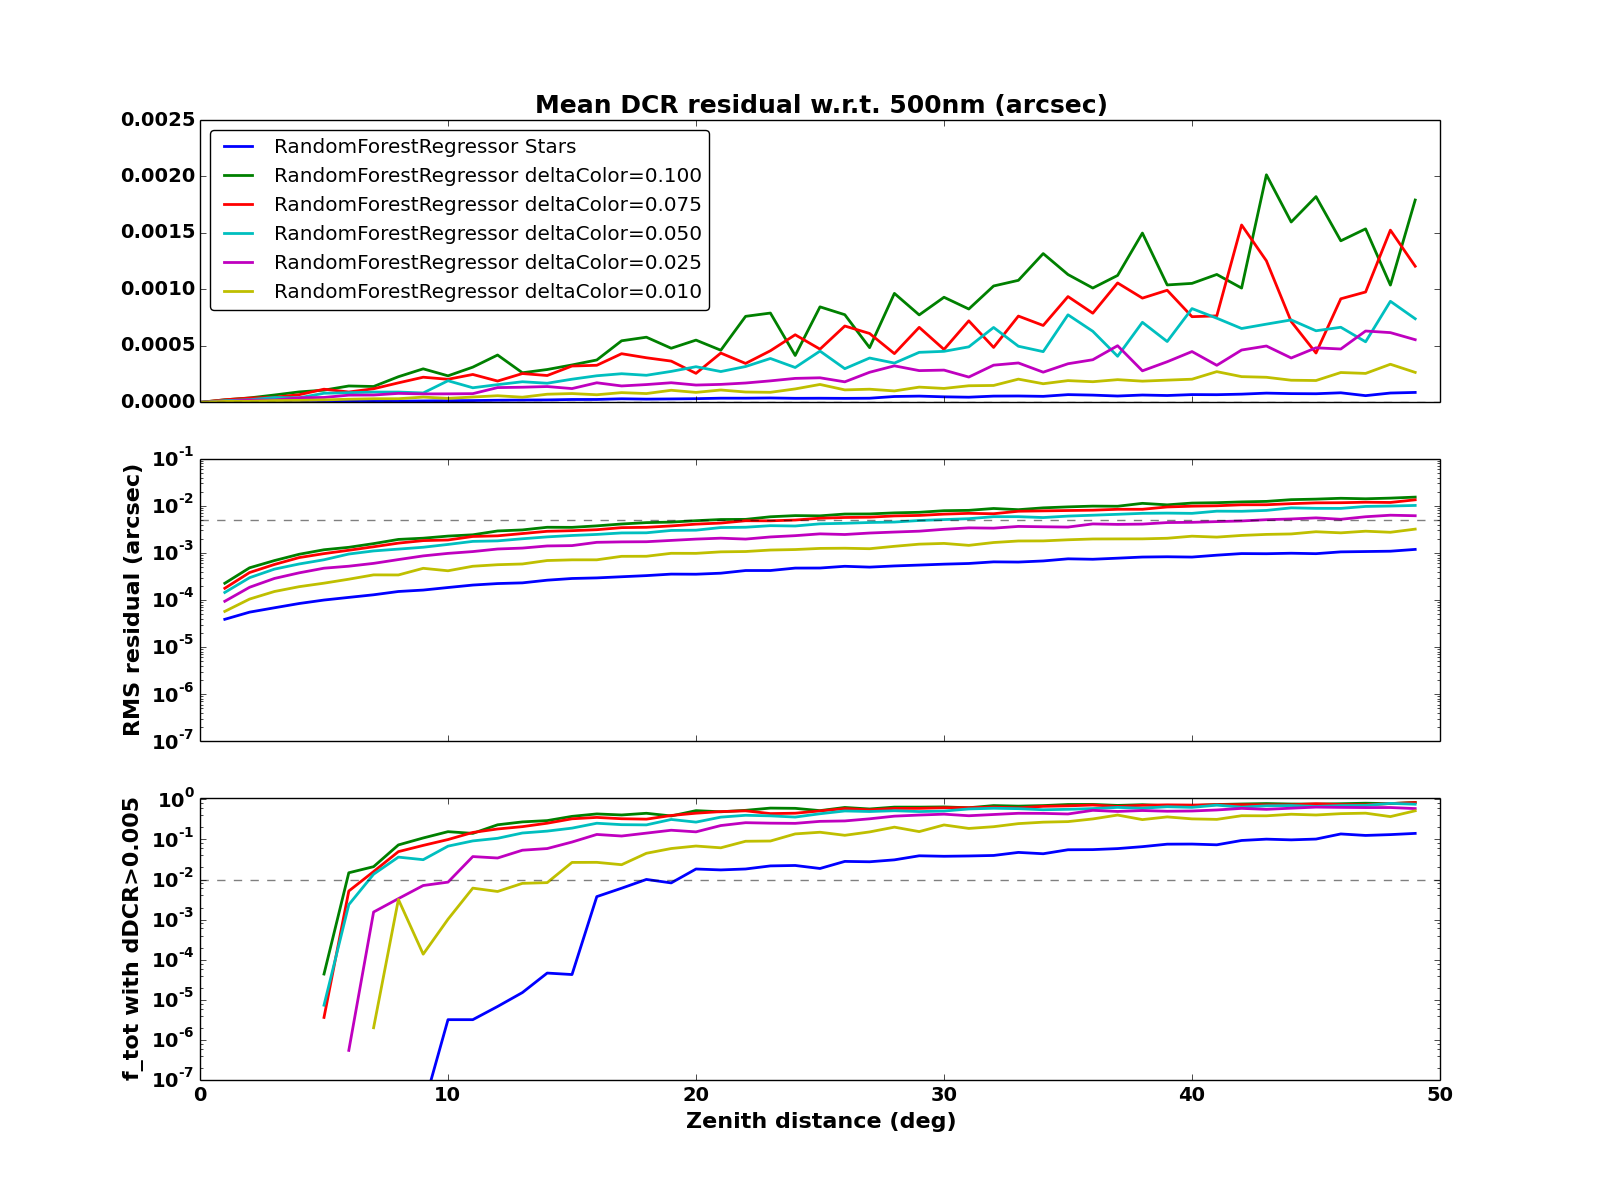
\includegraphics[width=\textwidth]{\figdir/DCR_u_deriv.png} }}
    \caption{{\bf Mapping Color Errors to DCR Misestimates}: This
      figure was created using the script {\tt
        python/calculateSedDcr4ML\_deriv.py}.}
    \label{dcrerr}
\end{figure}

\section{Summary}

%To create image subtraction templates, the effects of refraction
%should be ``taken out'' of the data before coaddition.  These effects
%should then be ``mimicked'' when mapping the template to the science
%image.  This requires both knowing the colors of sources (assumed to
%result from data release processing) and treating sources as a bundle
%of pixels of a given color (e.g. a footprint).

As this analysis has shown, the process of compensating for DCR will
be difficult in the $u$--band beyond 10 degrees zenith distance,
assuming $u-g$ source colors known to order 1\%.  The models examined
here do not have the power to generate an accurate prediction in this
passbands, in the presence of significant photometric noise.  The
large amplitude of DCR in this passband, along with the low
signal--to--noise expected in the $u$--band, will make this a
difficult task.

The results are significantly more optimistic in the $g$--band, where
1\% mismeasurements of source color yield approximately 1 object per
LSST sensor where the model will incorrectly predict the amplitude of
DCR by more than 5mas, beyond zenith distance of $\sim 25$ degrees.
In the $r$--band, there will be a similar population of objects with
10\% photometric errors, beyond zenith distance of $\sim 50$ degrees.
In the $iz$--bands, the amplitudes of DCR are small enough that there
is minimal dependence on the photometric quality.  We note that at
this fiducial offset of 5mas, 1\% of objects will show a DCR--based
dipole in 0.6'' seeing conditions.  For worse seeing, the mismatch
between model prediction and actual DCR amplitude can be larger before
yielding a 1\% chance of a dipole.

We note that this analysis has only been performed using the SEDs of
stellar objects.  It is {\it not} expected that a refraction or DCR
model generated using stars will be applicable to QSOs.  However,
objects with unusual SEDs may be identified based upon their
systematic residuals from stellar refraction models, and targeted for
further study.

\section{Additional Thoughts}

The requirements for the treatment of DCR in image subtraction must be
traced back to the creation of the image subtraction templates.  To
stack these images, the effects of DCR must be compensated for (or
``undone'') before coaddition/averaging.  To {\it not} do so will
introduce a systematic second moment to the effective template Psf
that will be source--color dependent.  While the baseline design is
for templates to be made at different seeings and airmasses, the
Winter 2014 work indicates that parallactic angle must be a third
variable to consider.  It is not clear if there will be enough data
early in the survey to make the requisite permutations of templates,
especially in the $u$ and $g$--bands.  This suggests that DCR may have
to be modeled and compensated for during the creation of the
templates, and then in the registration of the templates to the
science images.

One proposal is to model the effects of DCR at the pixel level, and
treat each footprint within an image as a bundle of pixels that have a
particular color.  Each bundle would then be remapped to a fiducial
(e.g. airmass=1) reference system with a color dependent term.
Coaddition would happen using these DCR--aware remapped images and the
models described above to predict this per--source additional offset.
The registration of such a template image to a new science image, with
its own DCR effects, would occur by mimicking the effects of DCR on
the template image pixel bundles, using the known source colors and
the airmass of the science image.  The background pixels (and the low
S/N sources within) would be remapped using an ``average'' color.

There are several difficulties with this process (which are not unique
to this pixel--based solution).  The first is that objects that change
in color will have a time--dependent DCR amplitude.  The second is
that the treatment of DCR in crowded fields, or of red/blue blends,
may not have a unique solution.  In this case even the consistent
treatment of these blended pixel bundles across epochs may not be
sufficient to completely undo for coaddition, and then mimic for
subtraction, the effects of DCR.  As a speculative note, it may be
possible to learn, or at least more tightly constrain, the optimal
deblending of pixels in the bundle using the time--series of images
and observations across the $ugr$--bands where DCR effects are
strongest.

Finally, the optimal treatment of DCR for faint (not detectable in
single--epoch images) sources will require an iterative approach,
where they are treated as background during the creation of detection
coadds.  After stacking and detection, they may be re--coadded using
the (approximate) colors that come from stacked or multi--fit
measurements.  The consequence of treating faint sources as background
will be loss in depth of detection in the coadd, for objects of
extreme color.  In all cases, a multi--epoch measurement package like
multi--fit will need to be DCR--aware to compensate for per--epoch
centroid shifts.

\bibliographystyle{apj}
\bibliography{refs}

\clearpage
\begin{appendices}
\section{Additional Figures}

\subsection{Modeling Refraction Using Broadband Colors \label{appx:rmodel}}
\begin{figure}[h]
    \centering
    \subfloat[$g$--band]{{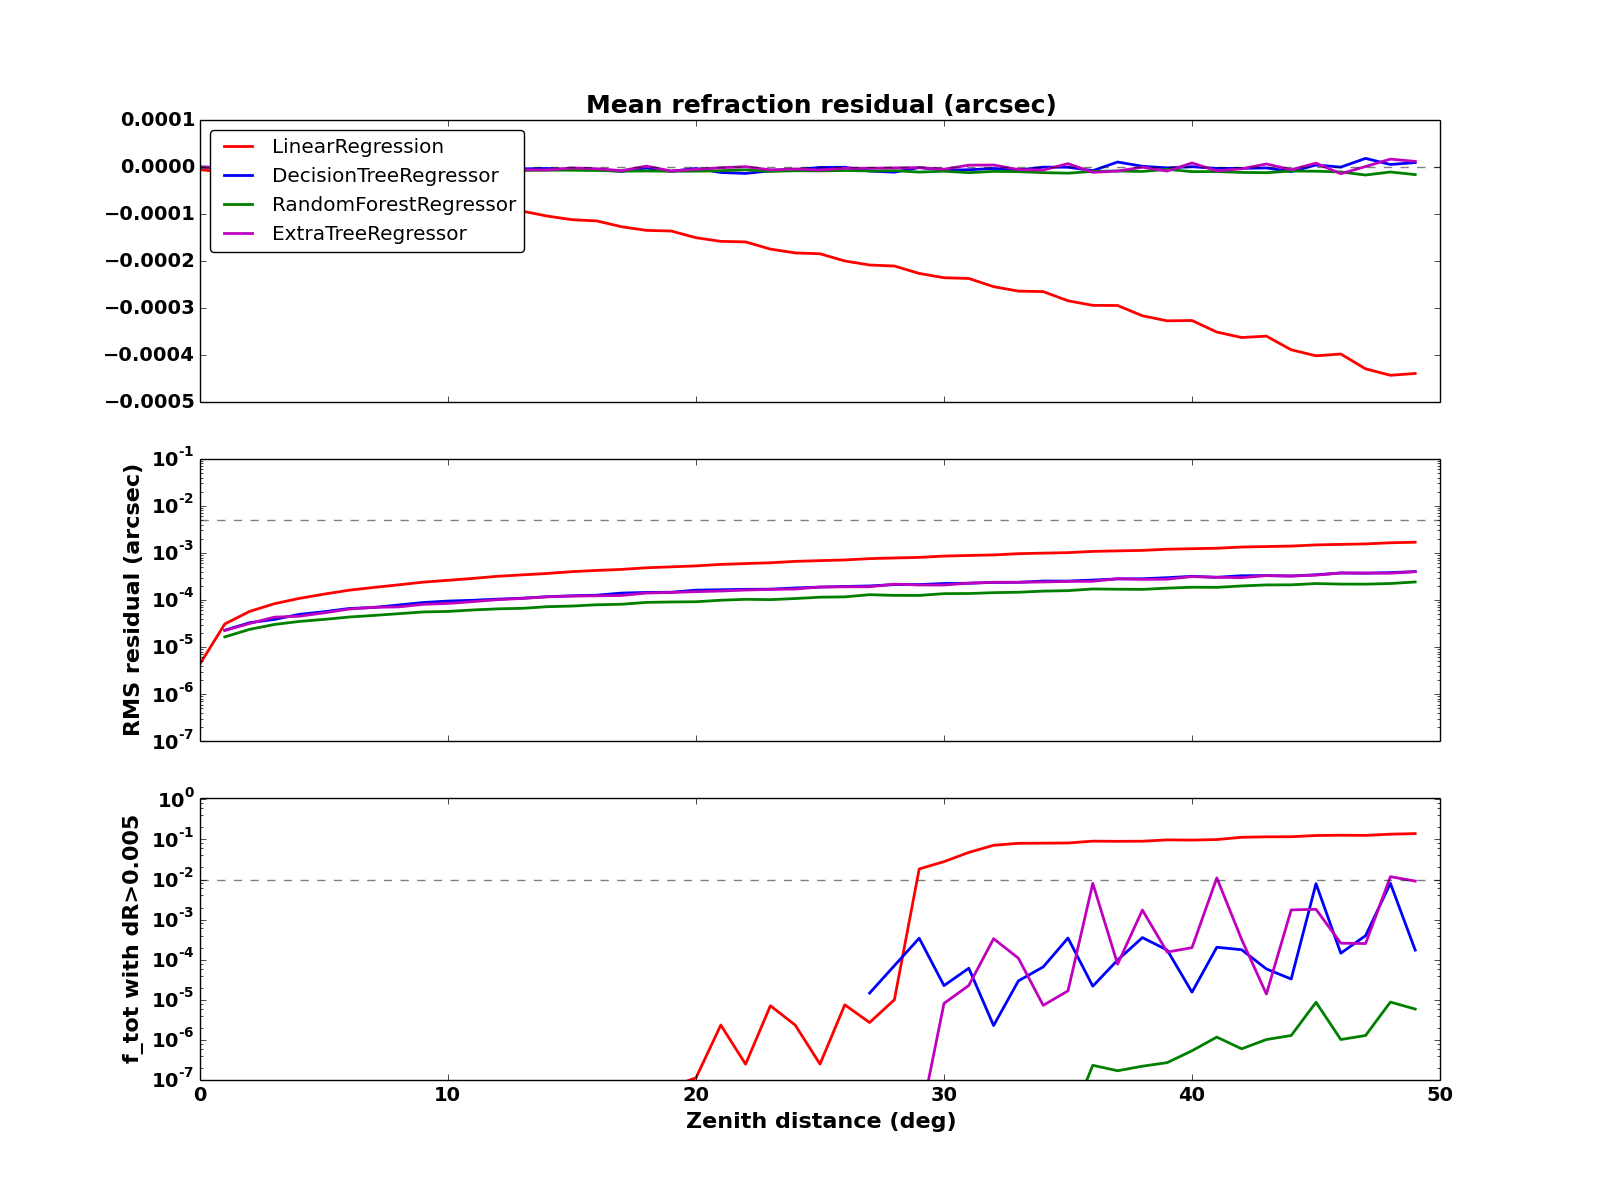
\includegraphics[width=\textwidth]{\figdir/R_g_A.png} }}
    \caption[]{{\bf Modeling Refraction Using Broadband Colors}: Continuation of Figure~\ref{rmodel}.}
    \label{rmodel2}
\end{figure}
\begin{figure}
    \ContinuedFloat 
    \centering
    \subfloat[$r$--band]{{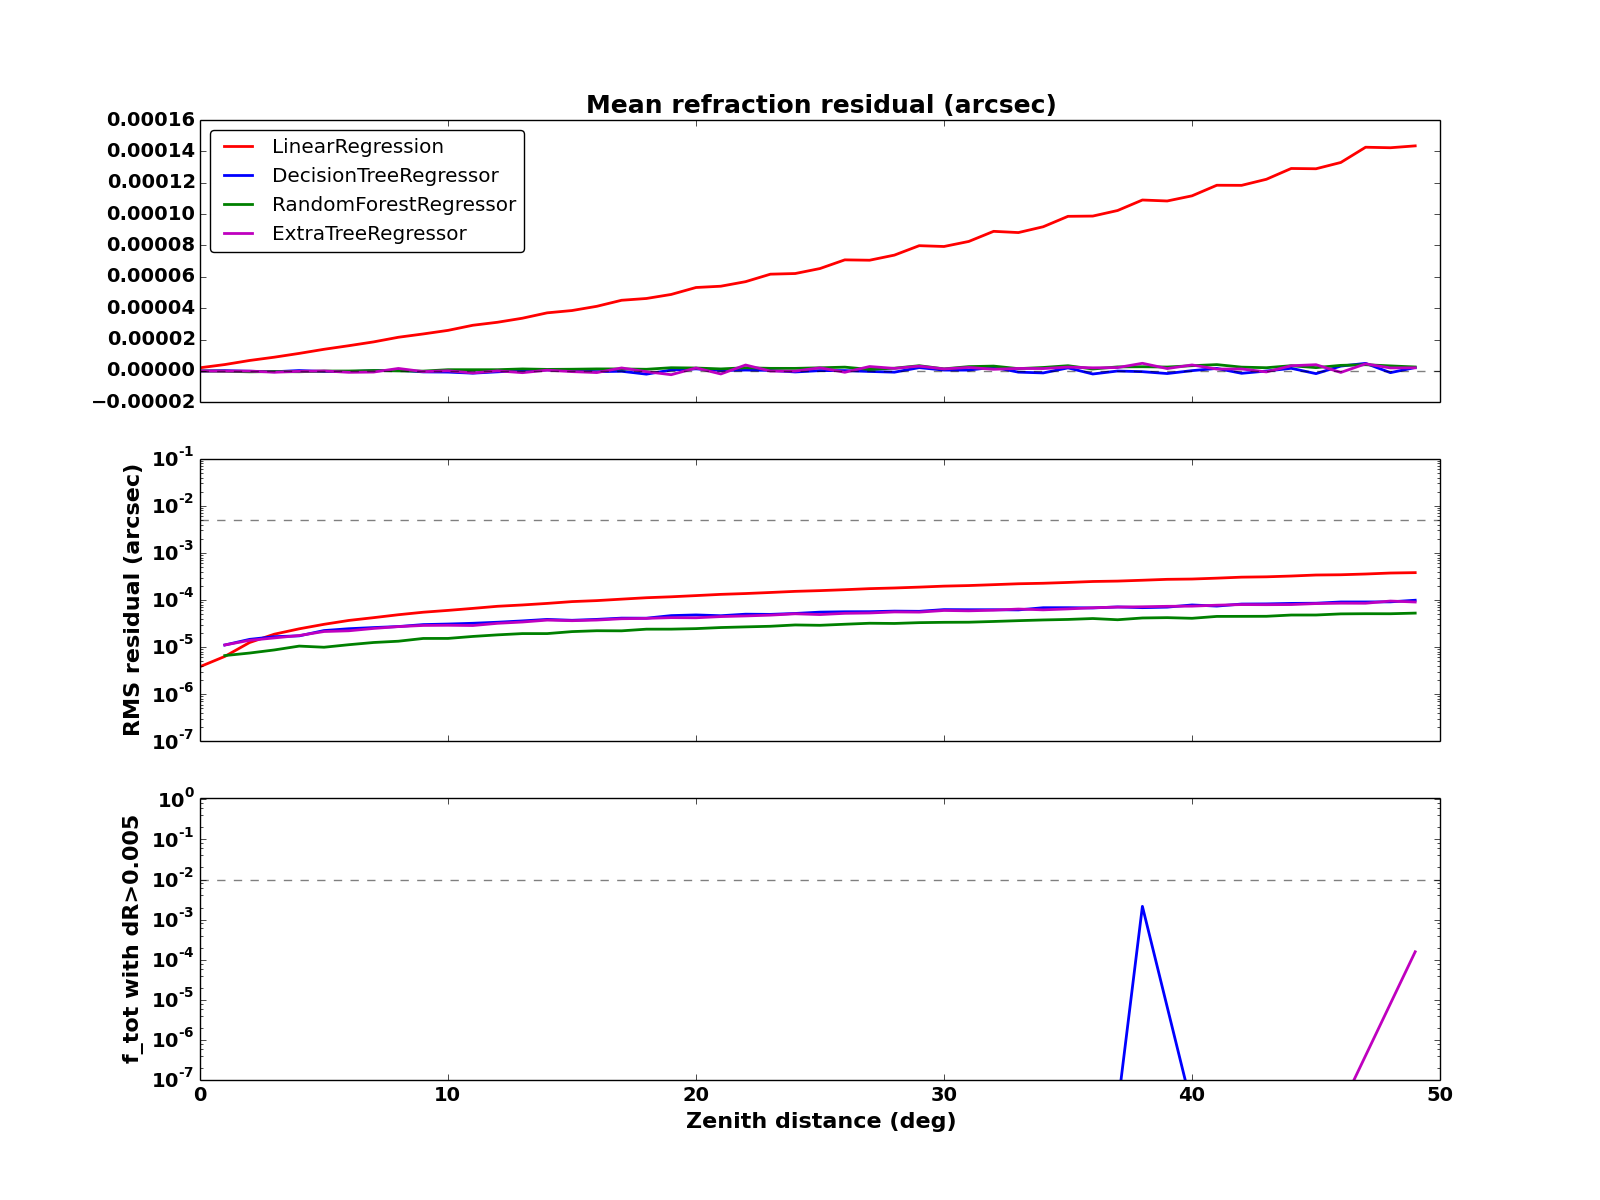
\includegraphics[width=\textwidth]{\figdir/R_r_A.png} }}
    \caption[]{{\bf Modeling Refraction Using Broadband Colors}: (cont)}
    \label{rmodel2}
\end{figure}
\begin{figure}
    \ContinuedFloat 
    \centering
    \subfloat[$i$--band]{{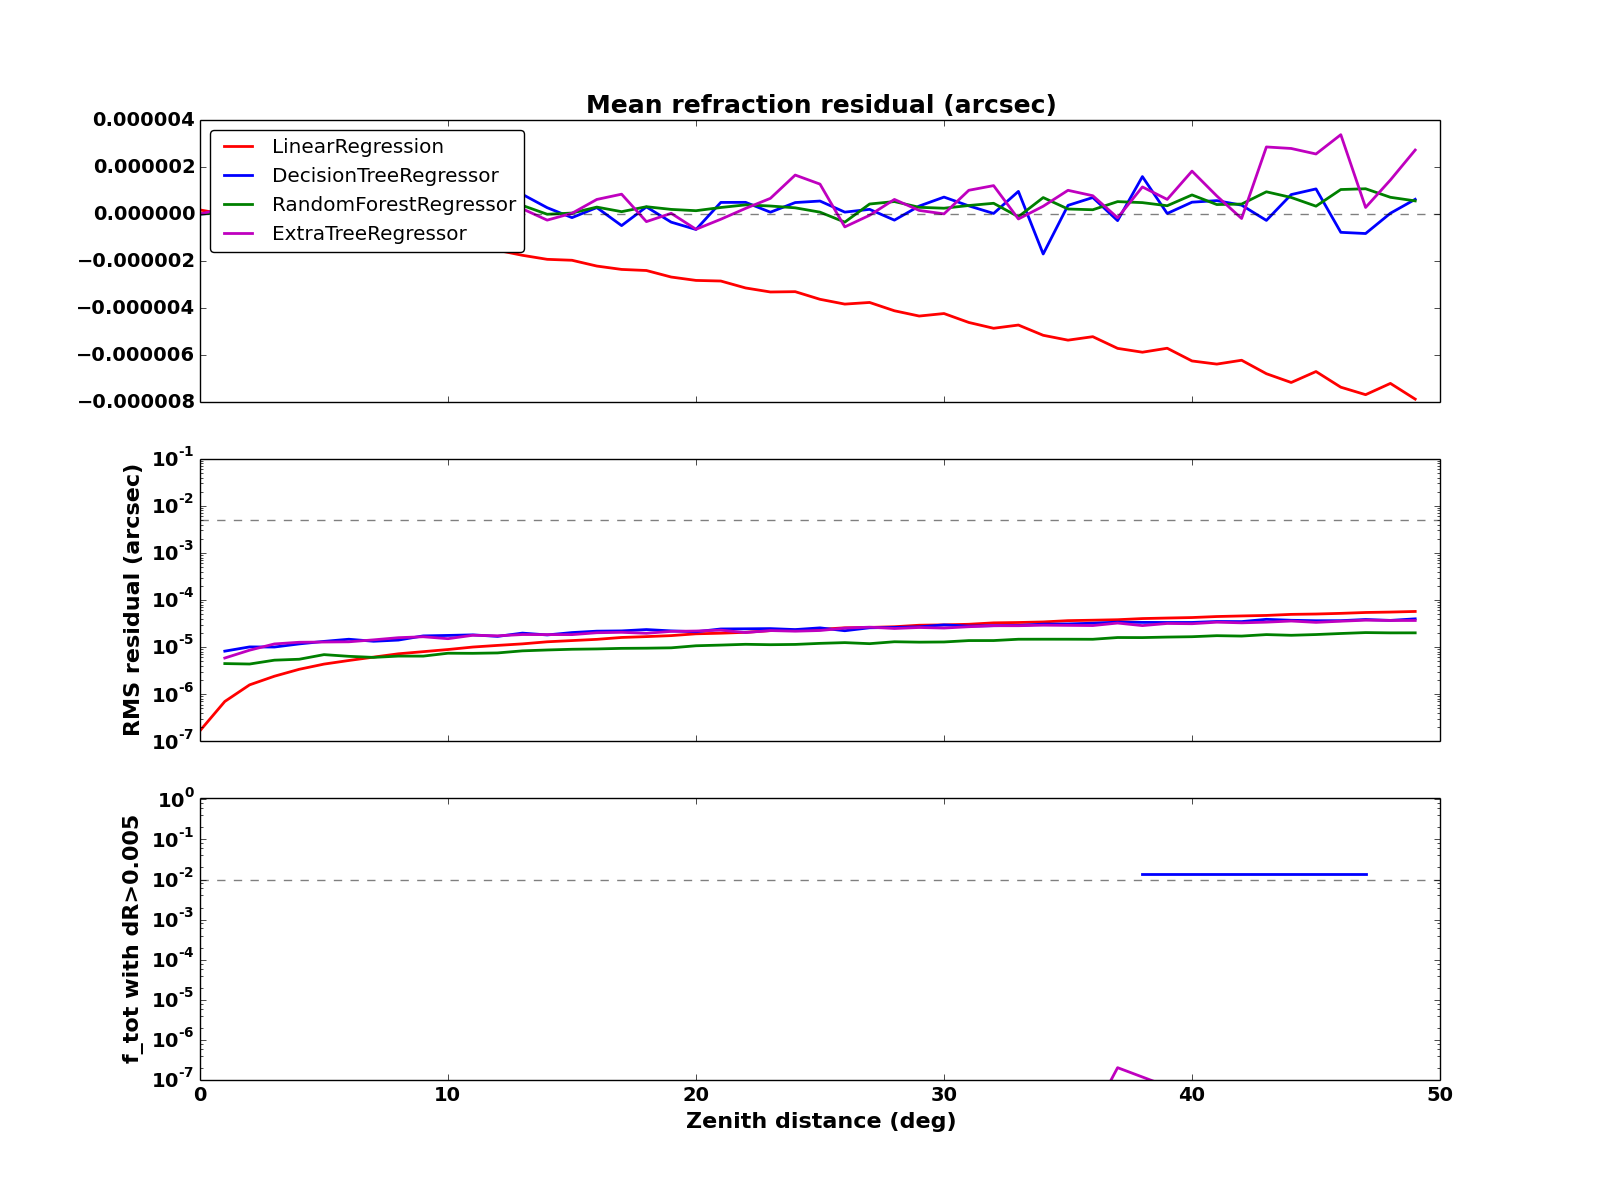
\includegraphics[width=\textwidth]{\figdir/R_i_A.png} }}
    \caption[]{{\bf Modeling Refraction Using Broadband Colors}: (cont)}
    \label{rmodel2}
\end{figure}
\begin{figure}
    \ContinuedFloat 
    \centering
    \subfloat[$z$--band]{{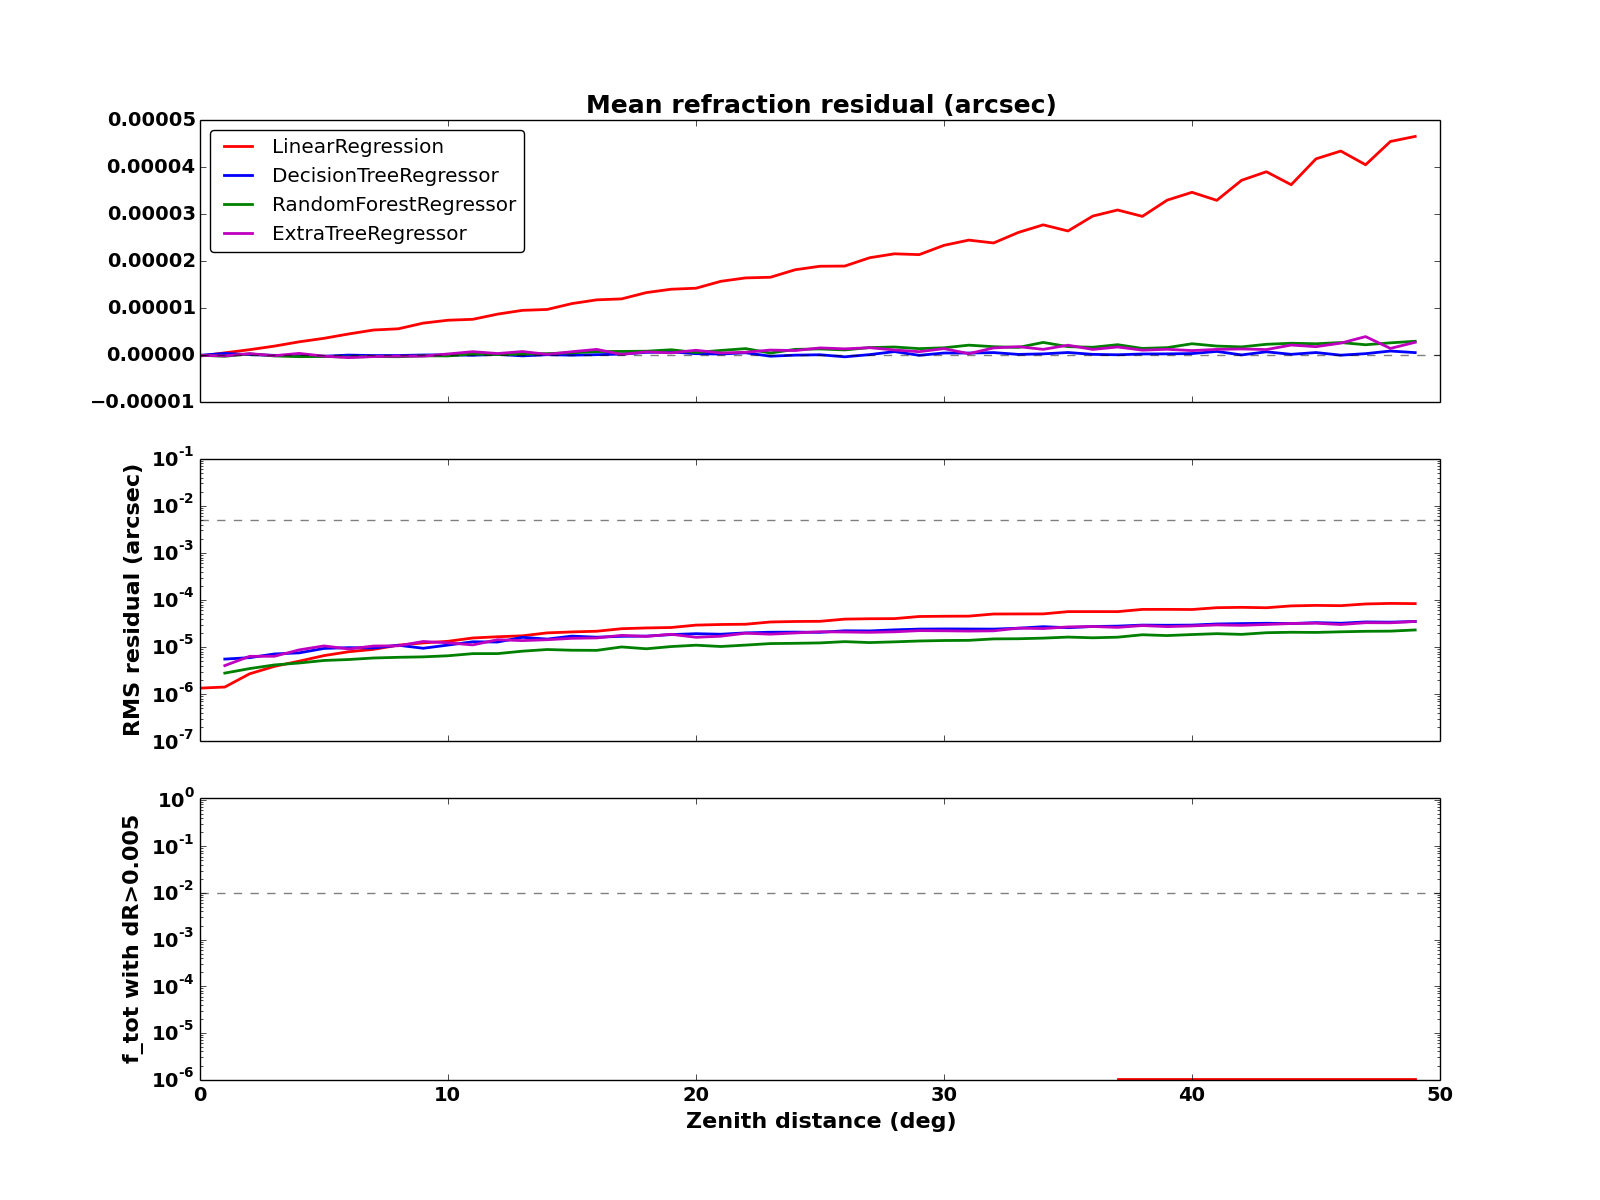
\includegraphics[width=\textwidth]{\figdir/R_z_A.png} }}
    \caption[]{{\bf Modeling Refraction Using Broadband Colors}: (cont)}
    \label{rmodel2}
\end{figure}
\clearpage

\subsection{Mapping Color Errors to Refraction Misestimates \label{appx:rerr}}
\begin{figure}[h]
    \centering
    \subfloat[$g$--band]{{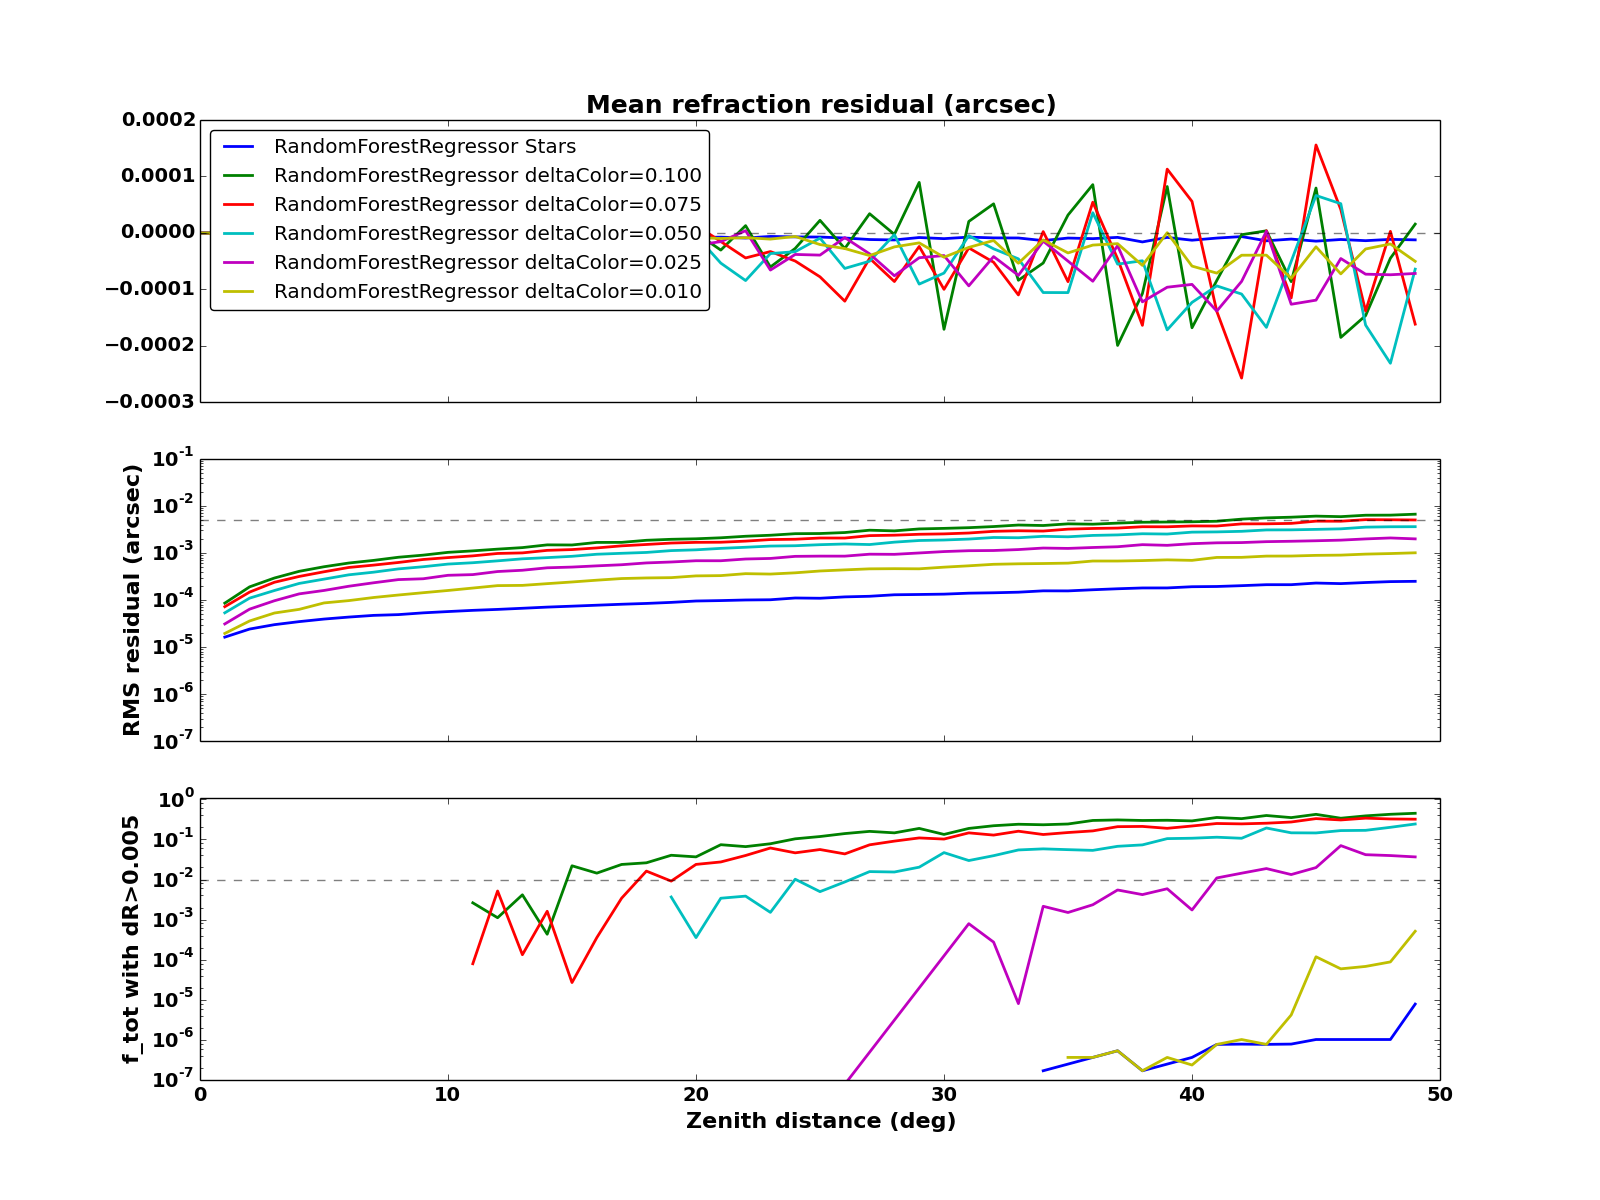
\includegraphics[width=\textwidth]{\figdir/R_g_deriv.png} }}
    \caption[]{{\bf Mapping Color Errors to Refraction Misestimates}:  Continuation of Figure~\ref{rerr}.}
    \label{rerr2}
\end{figure}
\begin{figure}
    \ContinuedFloat 
    \centering
    \subfloat[$r$--band]{{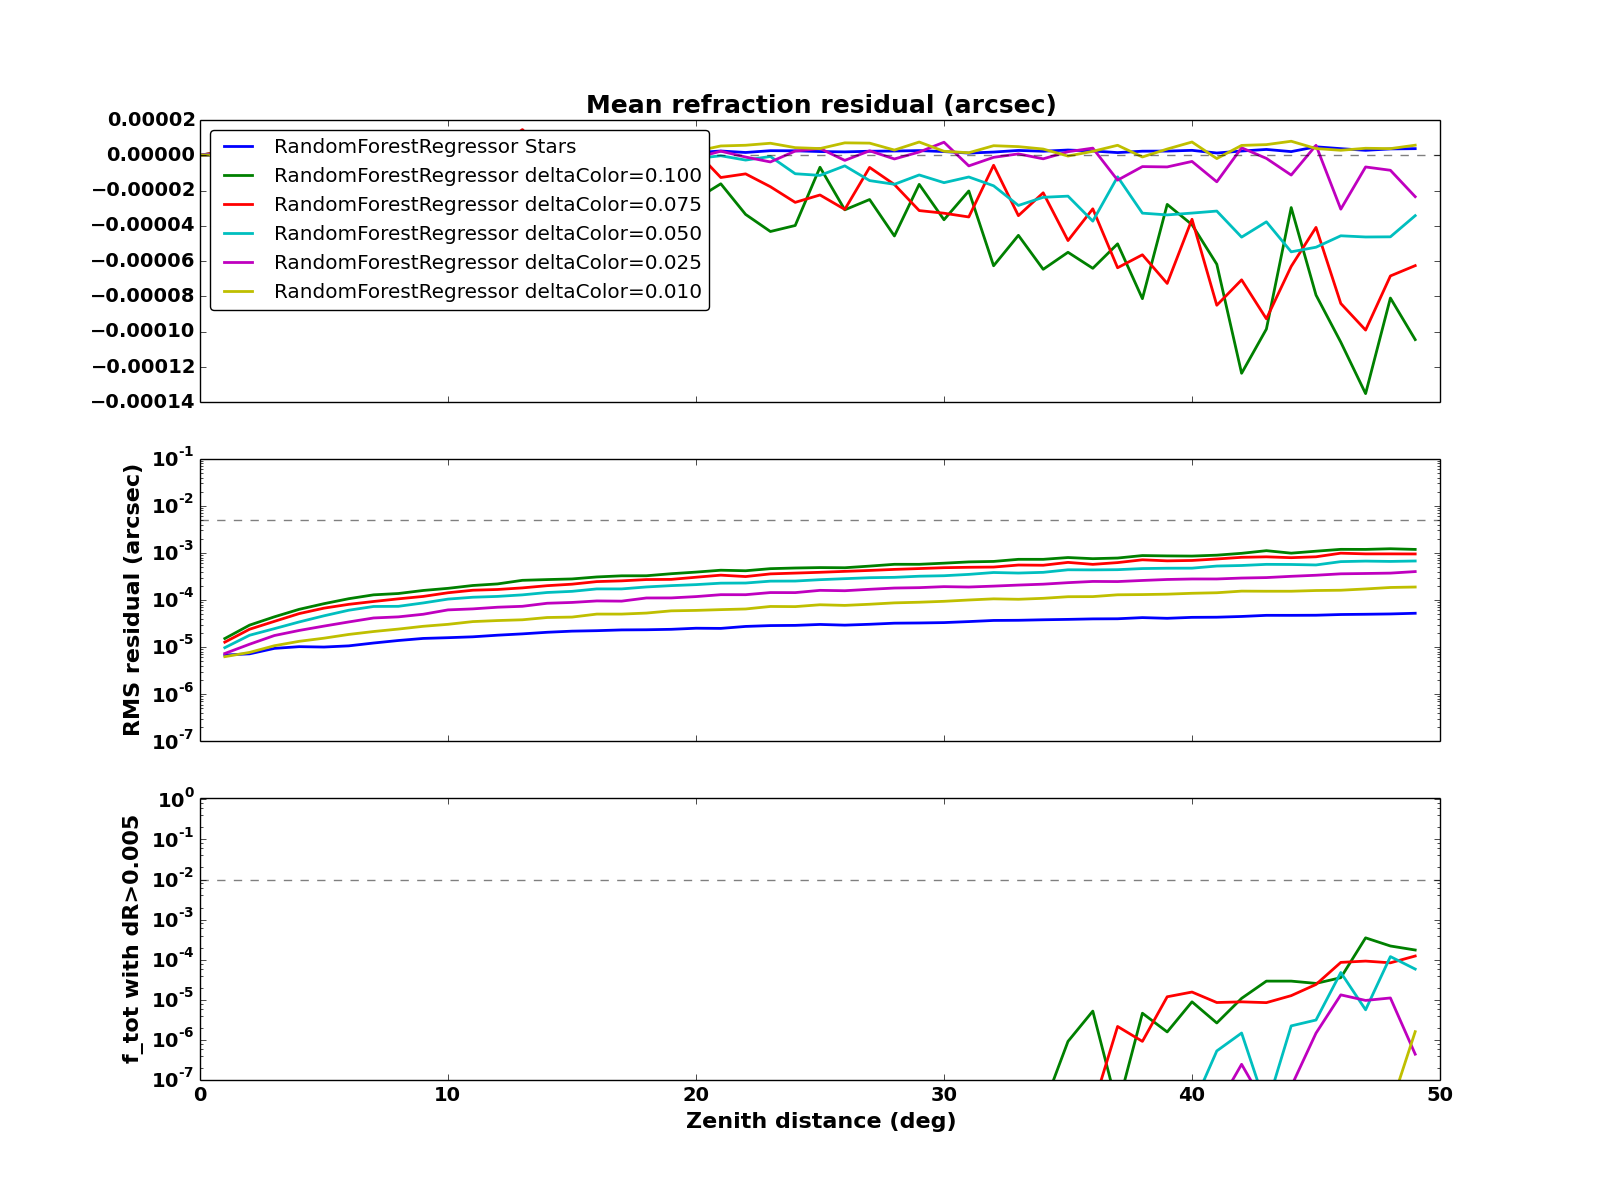
\includegraphics[width=\textwidth]{\figdir/R_r_deriv.png} }}
    \caption[]{{\bf Mapping Color Errors to Refraction Misestimates}: (cont)}
    \label{rerr2}
\end{figure}
\begin{figure}
    \ContinuedFloat 
    \centering
    \subfloat[$i$--band]{{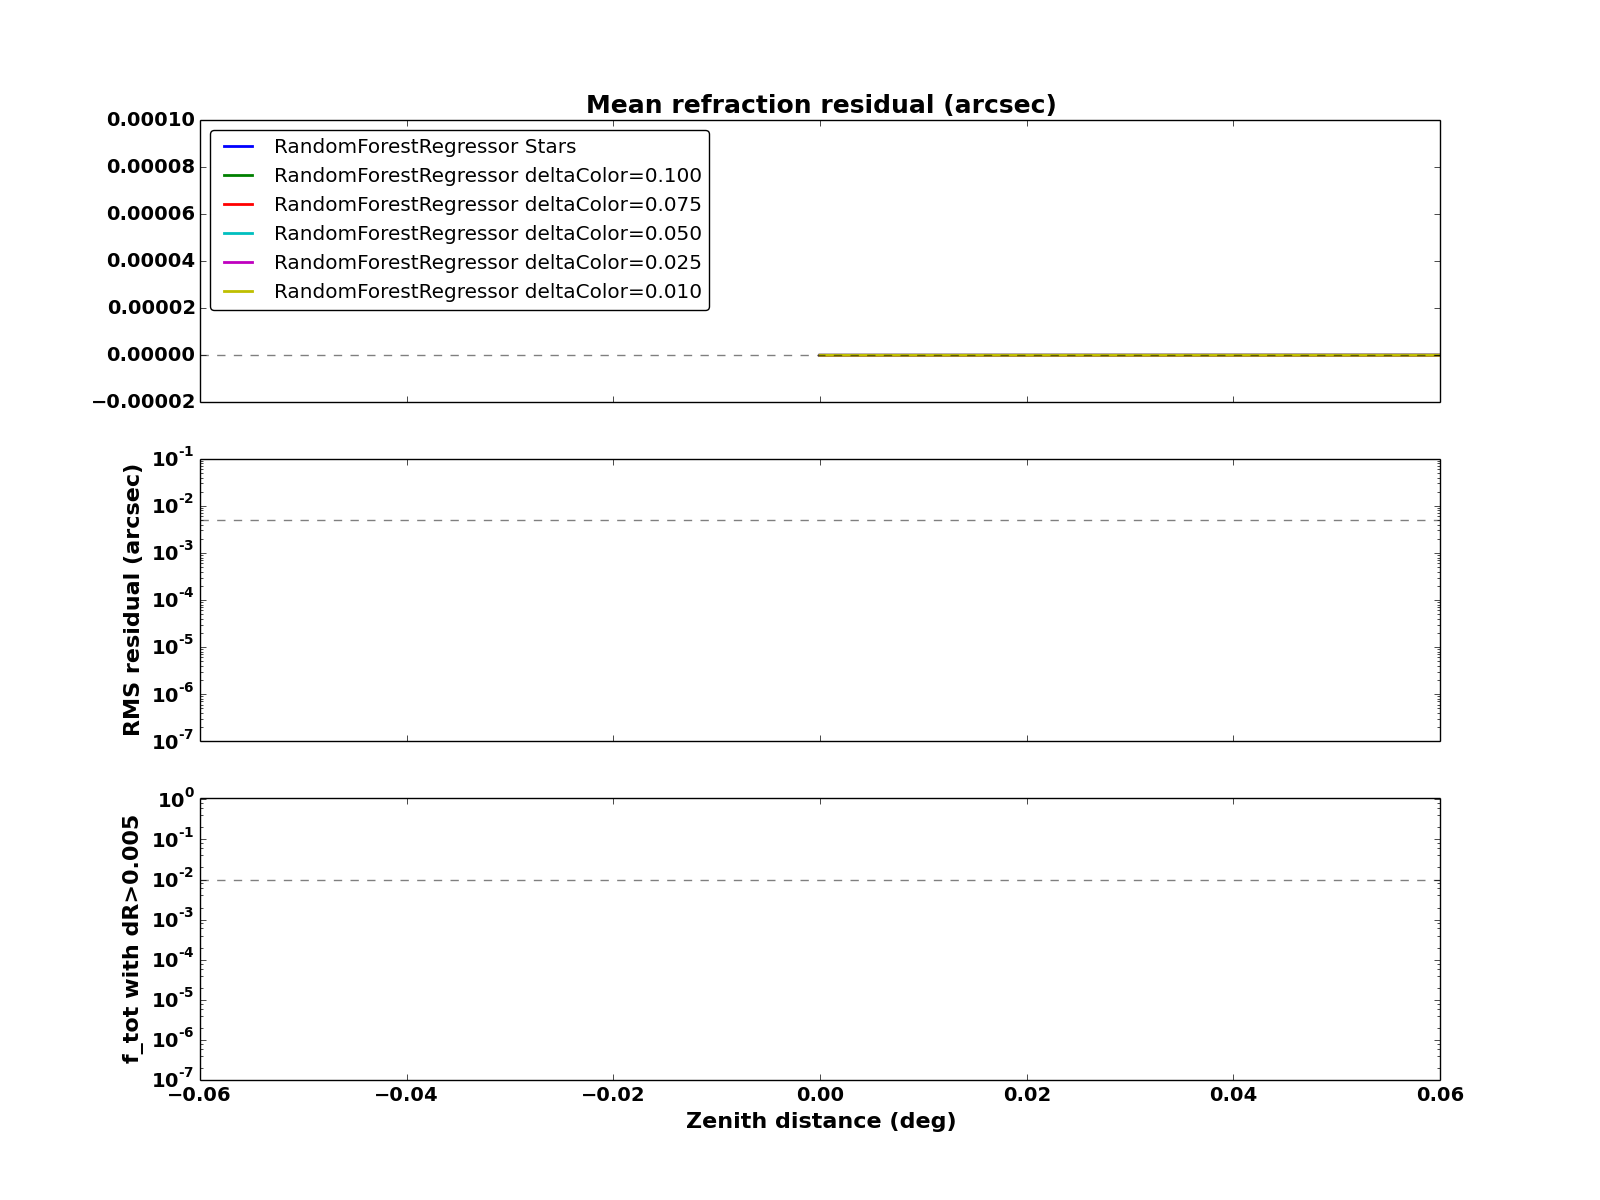
\includegraphics[width=\textwidth]{\figdir/R_i_deriv.png} }}
    \caption[]{{\bf Mapping Color Errors to Refraction Misestimates}: (cont)}
    \label{rerr2}
\end{figure}
\begin{figure}
    \ContinuedFloat 
    \centering
    \subfloat[$z$--band]{{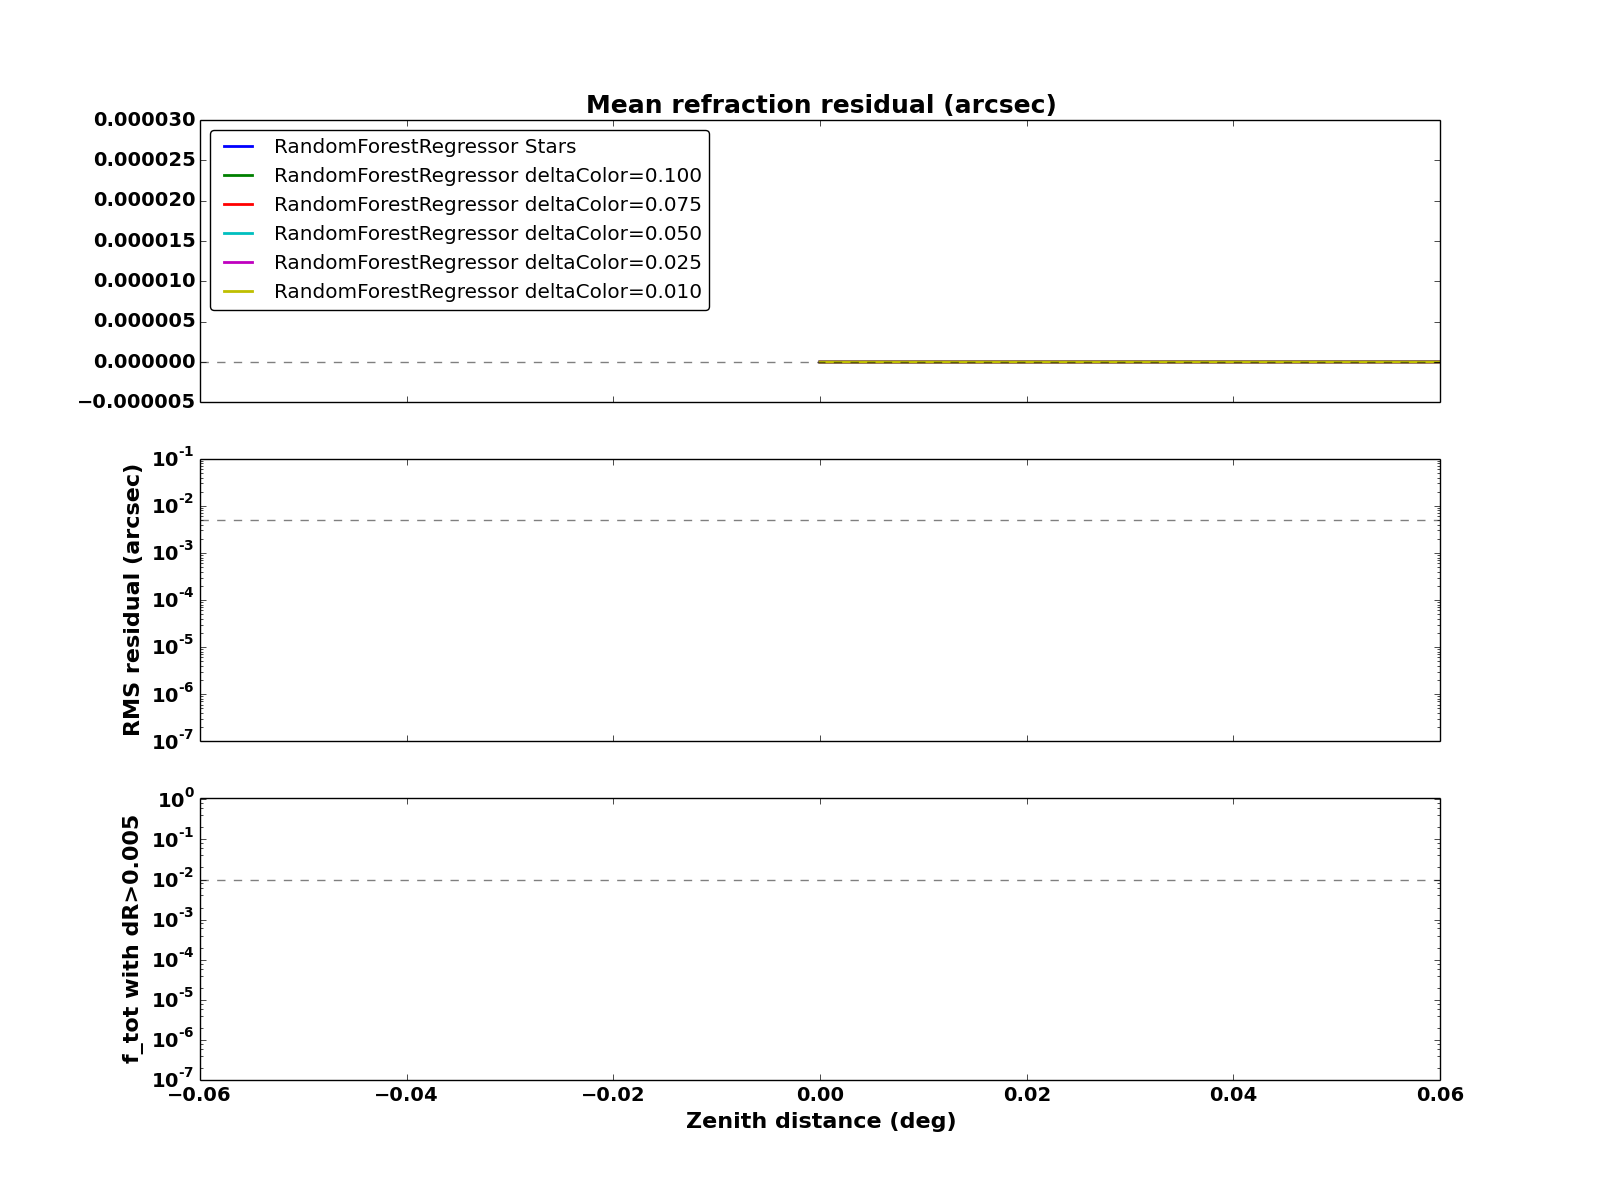
\includegraphics[width=\textwidth]{\figdir/R_z_deriv.png} }}
    \caption[]{{\bf Mapping Color Errors to Refraction Misestimates}: (cont)}
    \label{rerr2}
\end{figure}
\clearpage

\subsection{Modeling DCR Using Broadband Colors \label{appx:dcrmodel}}
\begin{figure}[h]
    \centering
    \subfloat[$g$--band]{{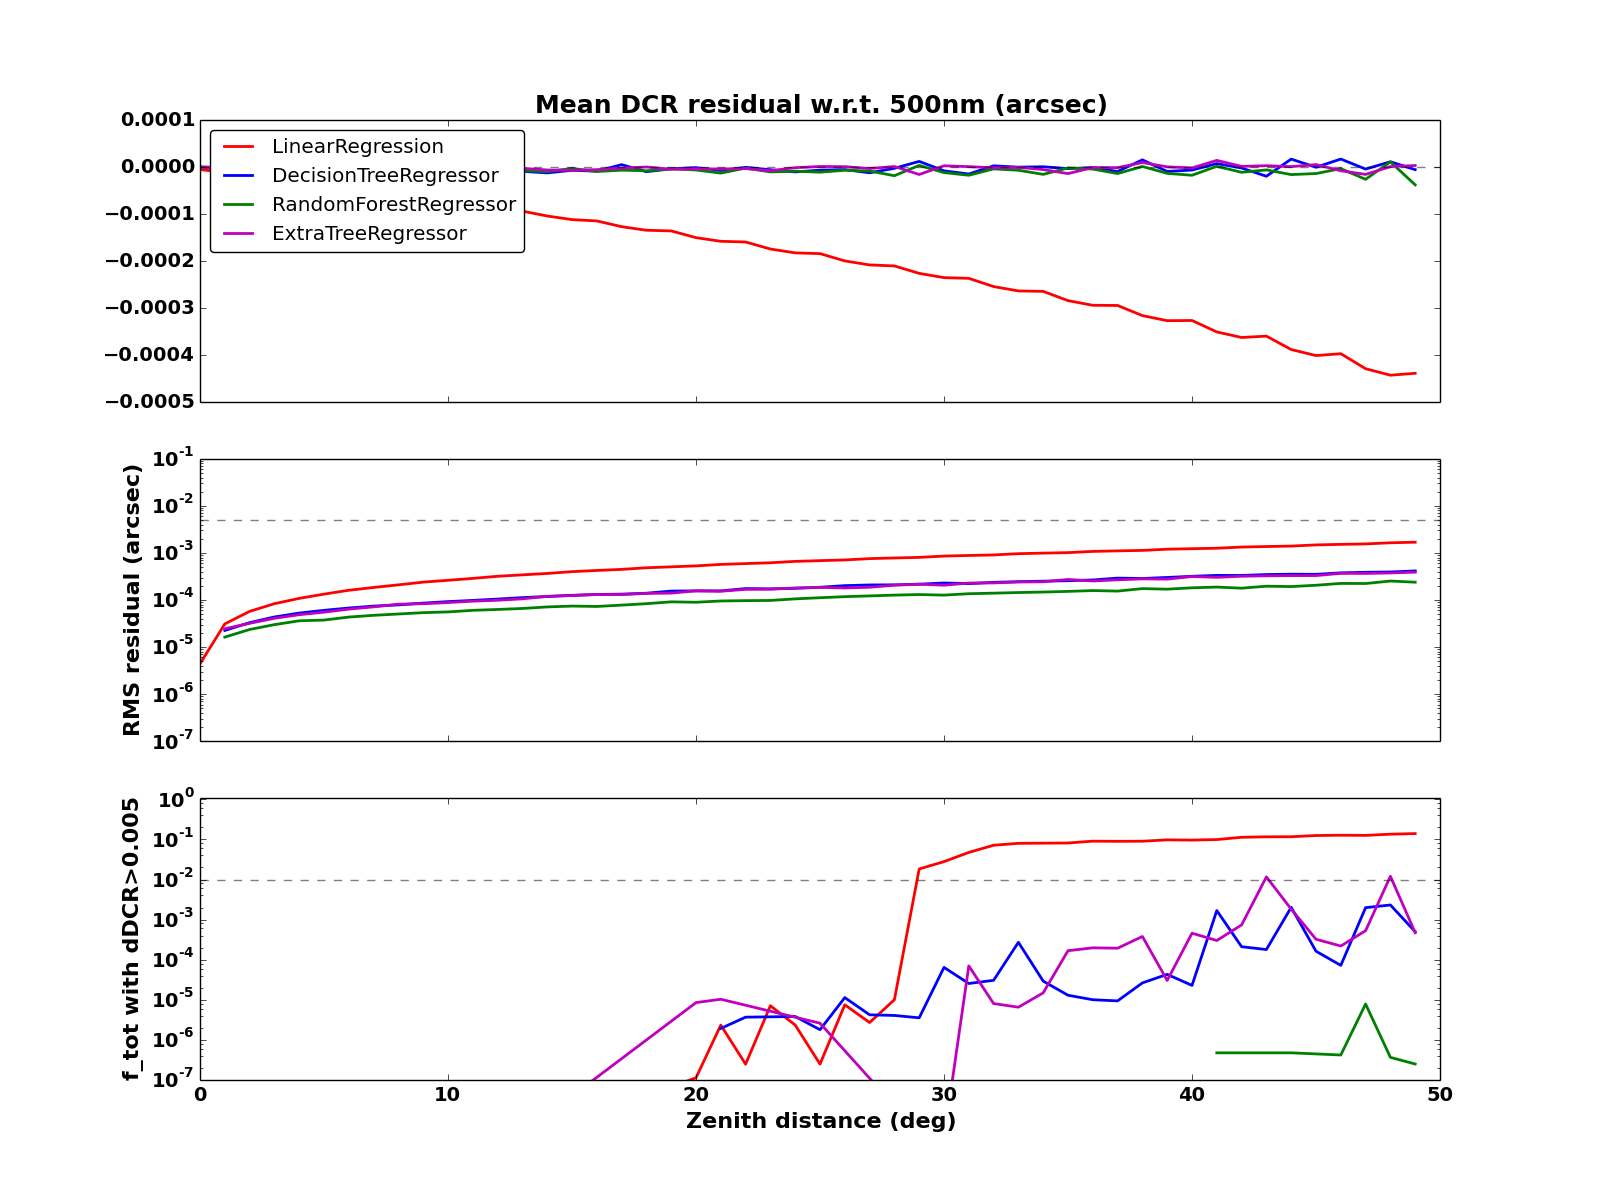
\includegraphics[width=\textwidth]{\figdir/DCR_g_A.png} }}
    \caption[]{{\bf Modeling DCR Using Broadband Colors}: Continuation of Figure~\ref{dcrmodel}.}
    \label{dcrmodel2}
\end{figure}
\begin{figure}
    \ContinuedFloat 
    \centering
    \subfloat[$r$--band]{{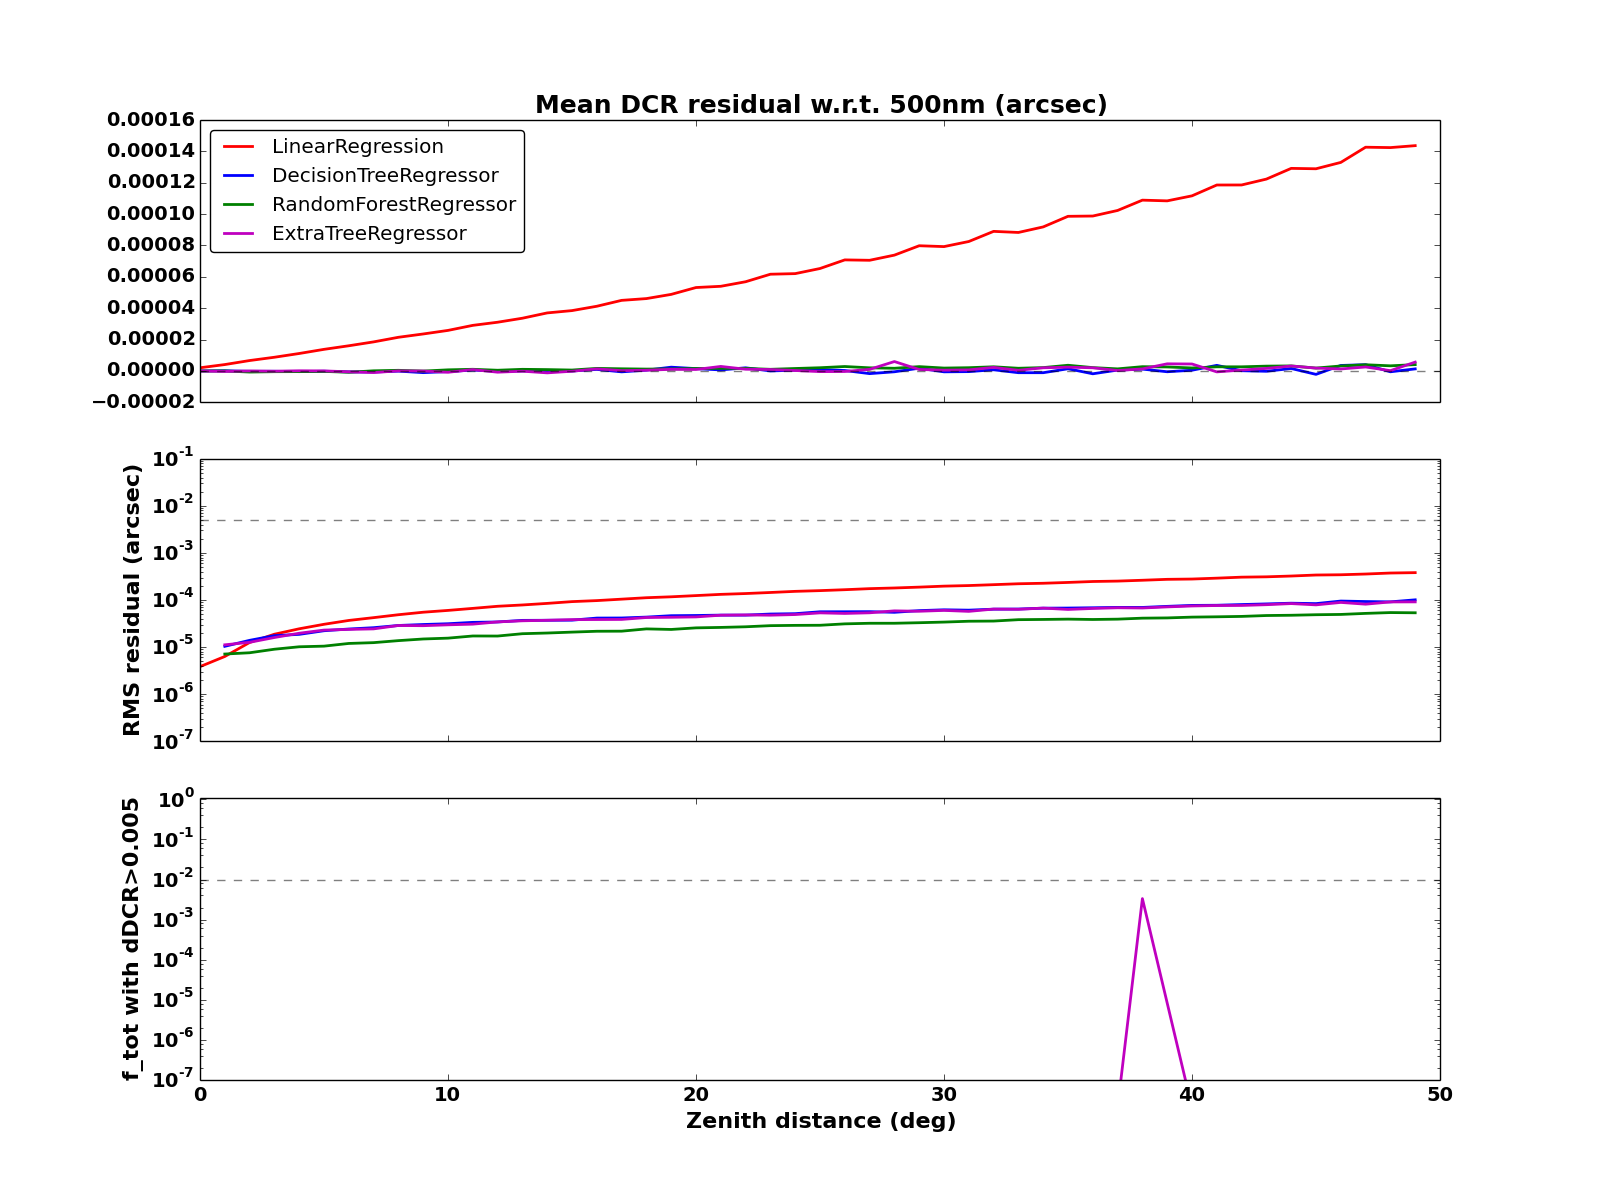
\includegraphics[width=\textwidth]{\figdir/DCR_r_A.png} }}
    \caption[]{{\bf Modeling DCR Using Broadband Colors}: (cont)}
    \label{dcrmodel2}
\end{figure}
\begin{figure}
    \ContinuedFloat 
    \centering
    \subfloat[$i$--band]{{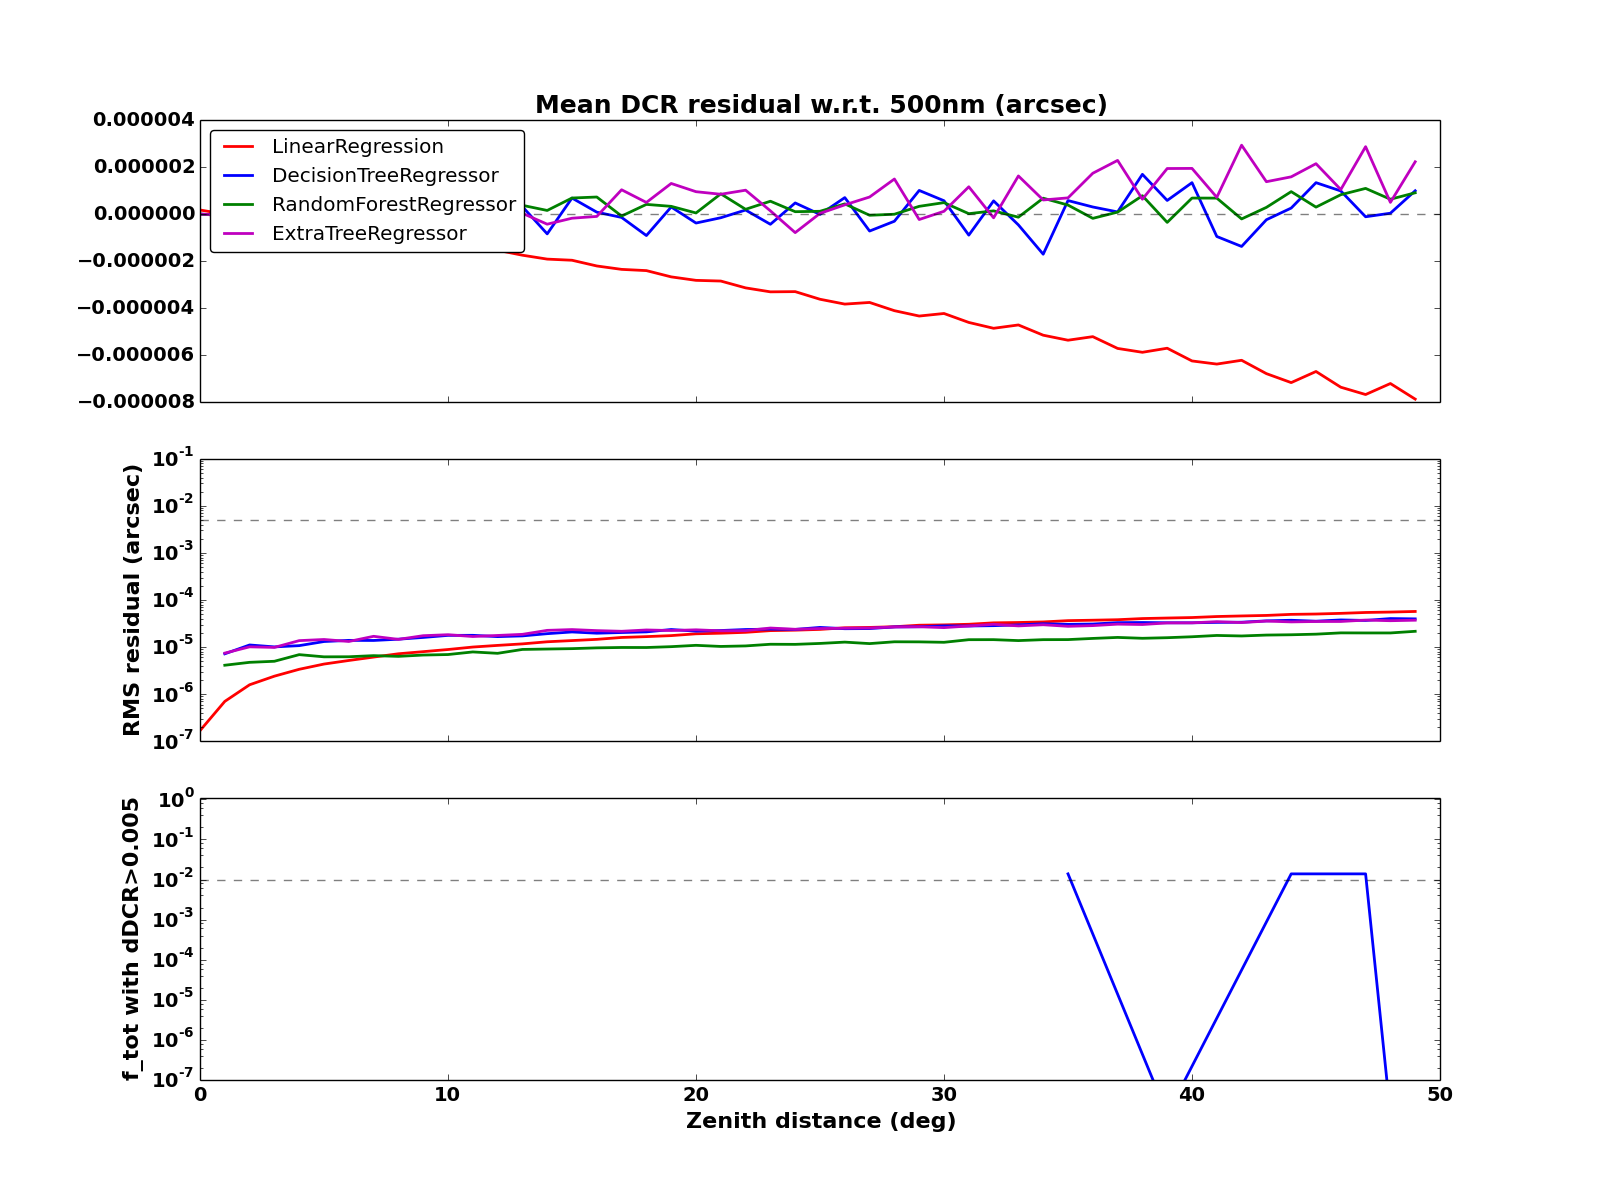
\includegraphics[width=\textwidth]{\figdir/DCR_i_A.png} }}
    \caption[]{{\bf Modeling DCR Using Broadband Colors}: (cont)}
    \label{dcrmodel2}
\end{figure}
\begin{figure}
    \ContinuedFloat 
    \centering
    \subfloat[$z$--band]{{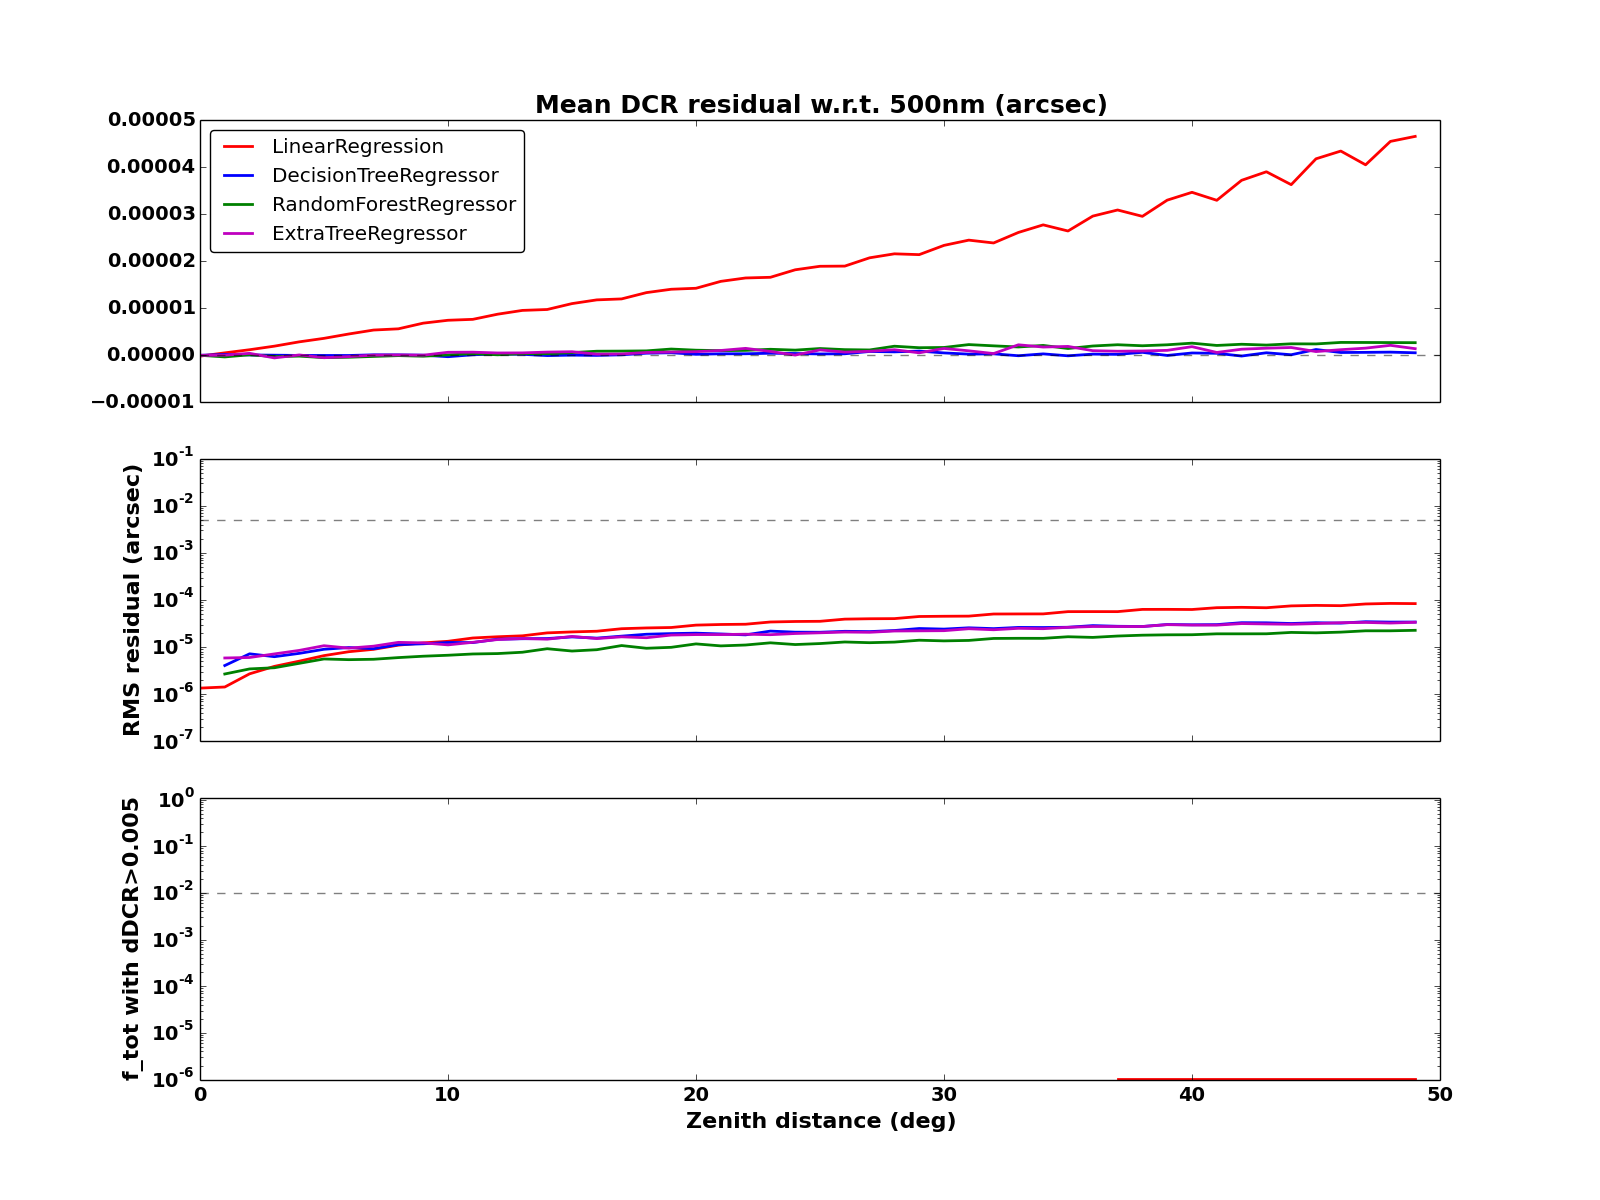
\includegraphics[width=\textwidth]{\figdir/DCR_z_A.png} }}
    \caption[]{{\bf Modeling DCR Using Broadband Colors}: (cont)}
    \label{dcrmodel2}
\end{figure}
\clearpage

\subsection{Mapping Color Errors to DCR Misestimates \label{appx:dcrerr}}
\begin{figure}[h]
    \centering
    \subfloat[$g$--band]{{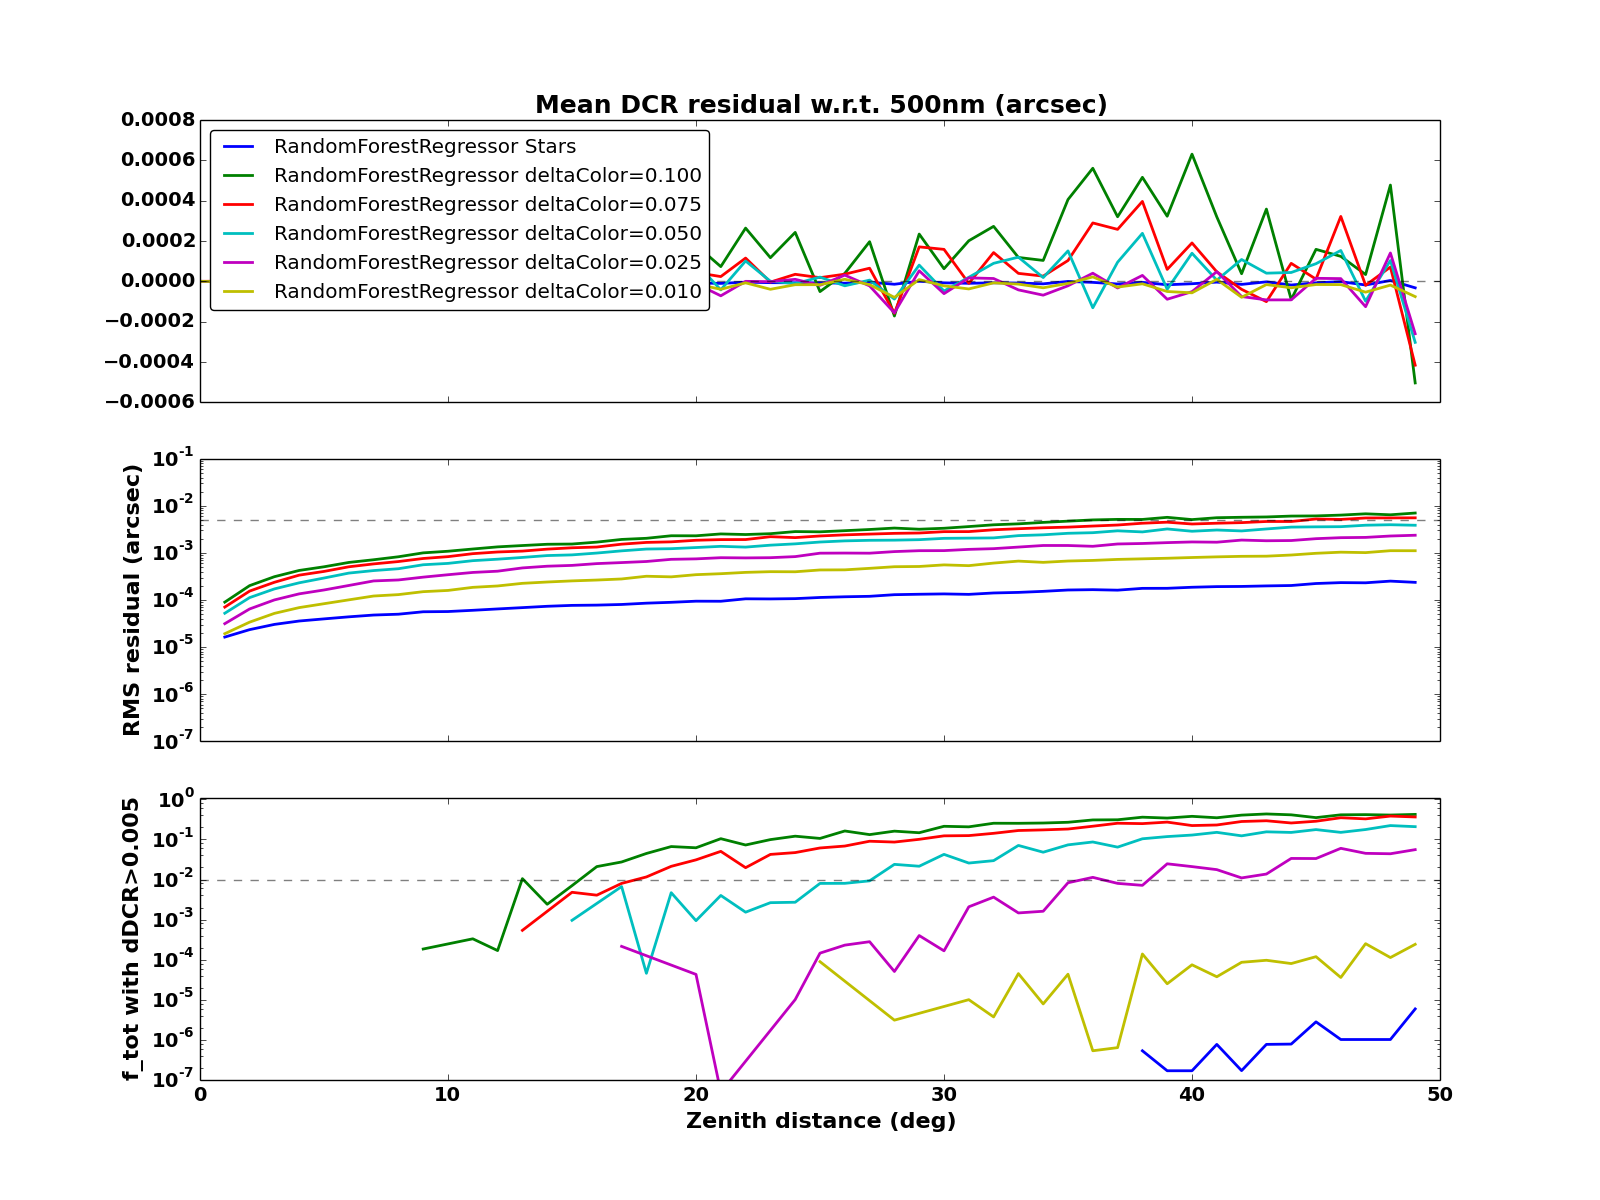
\includegraphics[width=\textwidth]{\figdir/DCR_g_deriv.png} }}
    \caption[]{{\bf Mapping Color Errors to DCR Misestimates}: Continuation of Figure~\ref{dcrerr}.}
    \label{dcrerr2}
\end{figure}
\begin{figure}
    \ContinuedFloat 
    \centering
    \subfloat[$r$--band]{{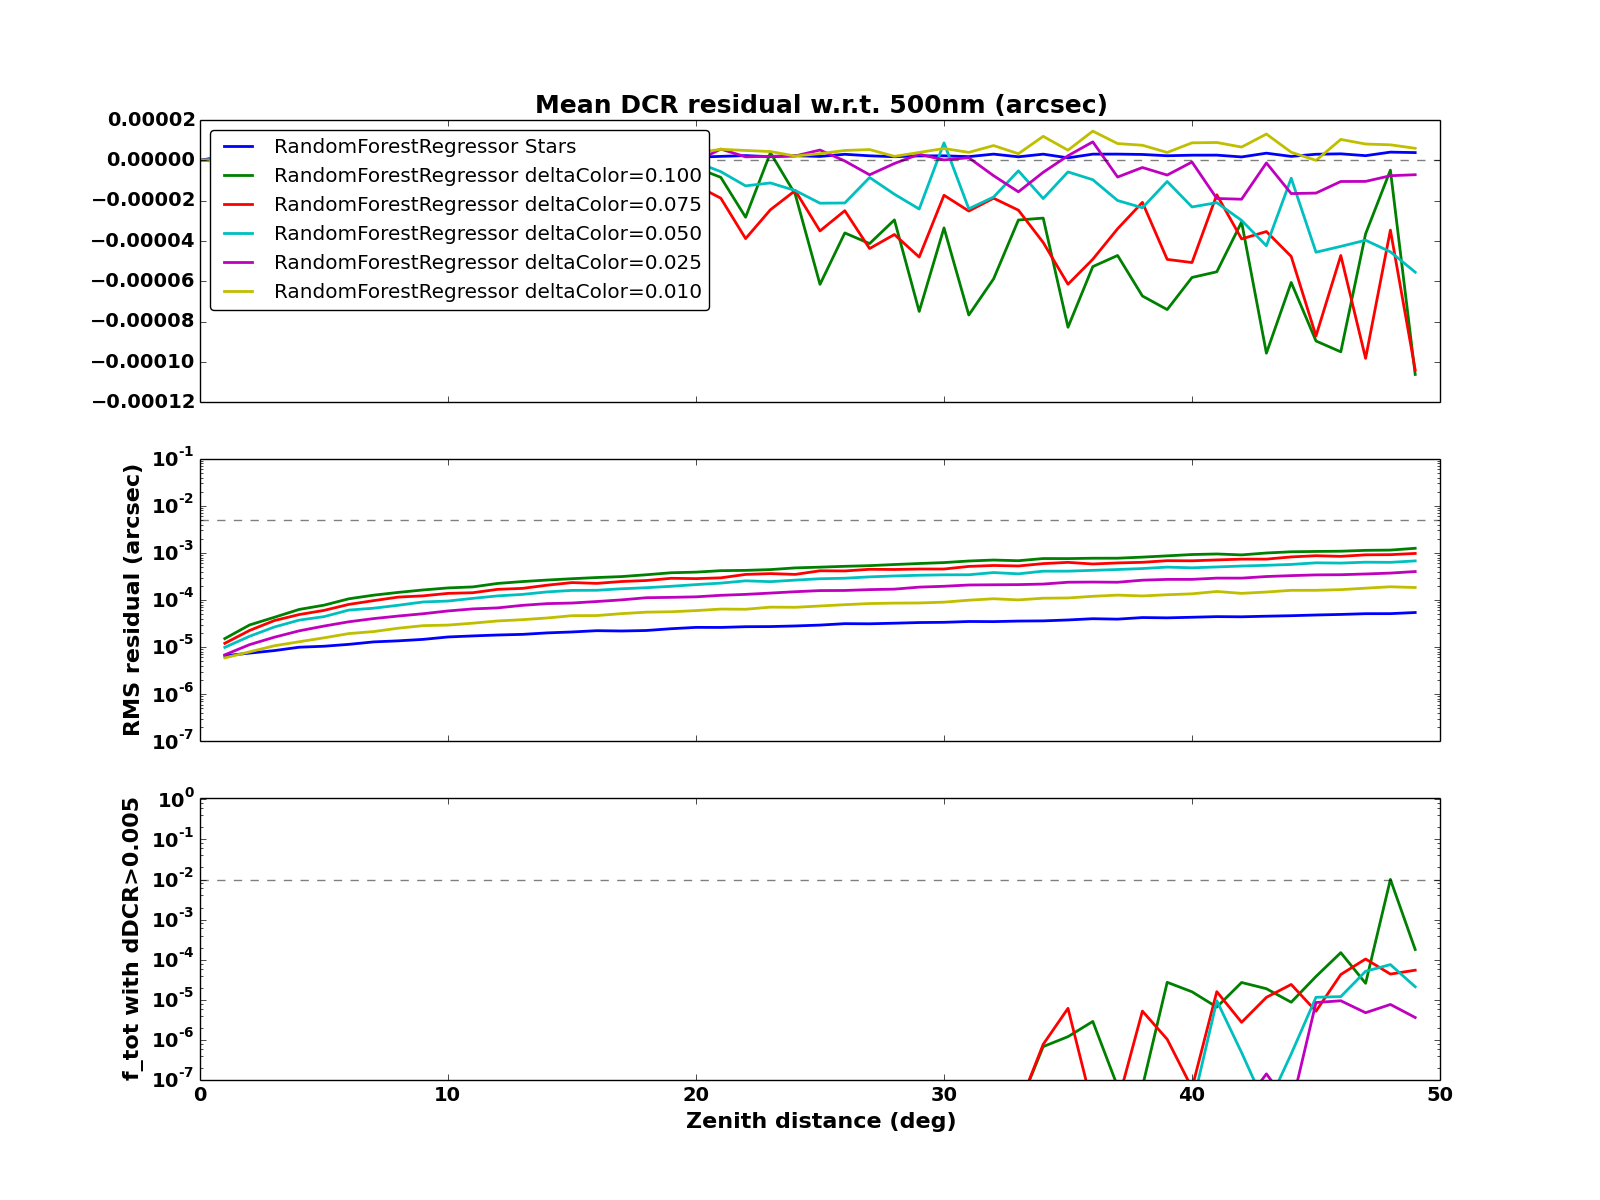
\includegraphics[width=\textwidth]{\figdir/DCR_r_deriv.png} }}
    \caption[]{{\bf Mapping Color Errors to DCR Misestimates}: (cont)}
    \label{dcrerr2}
\end{figure}
\begin{figure}
    \ContinuedFloat 
    \centering
    \subfloat[$i$--band]{{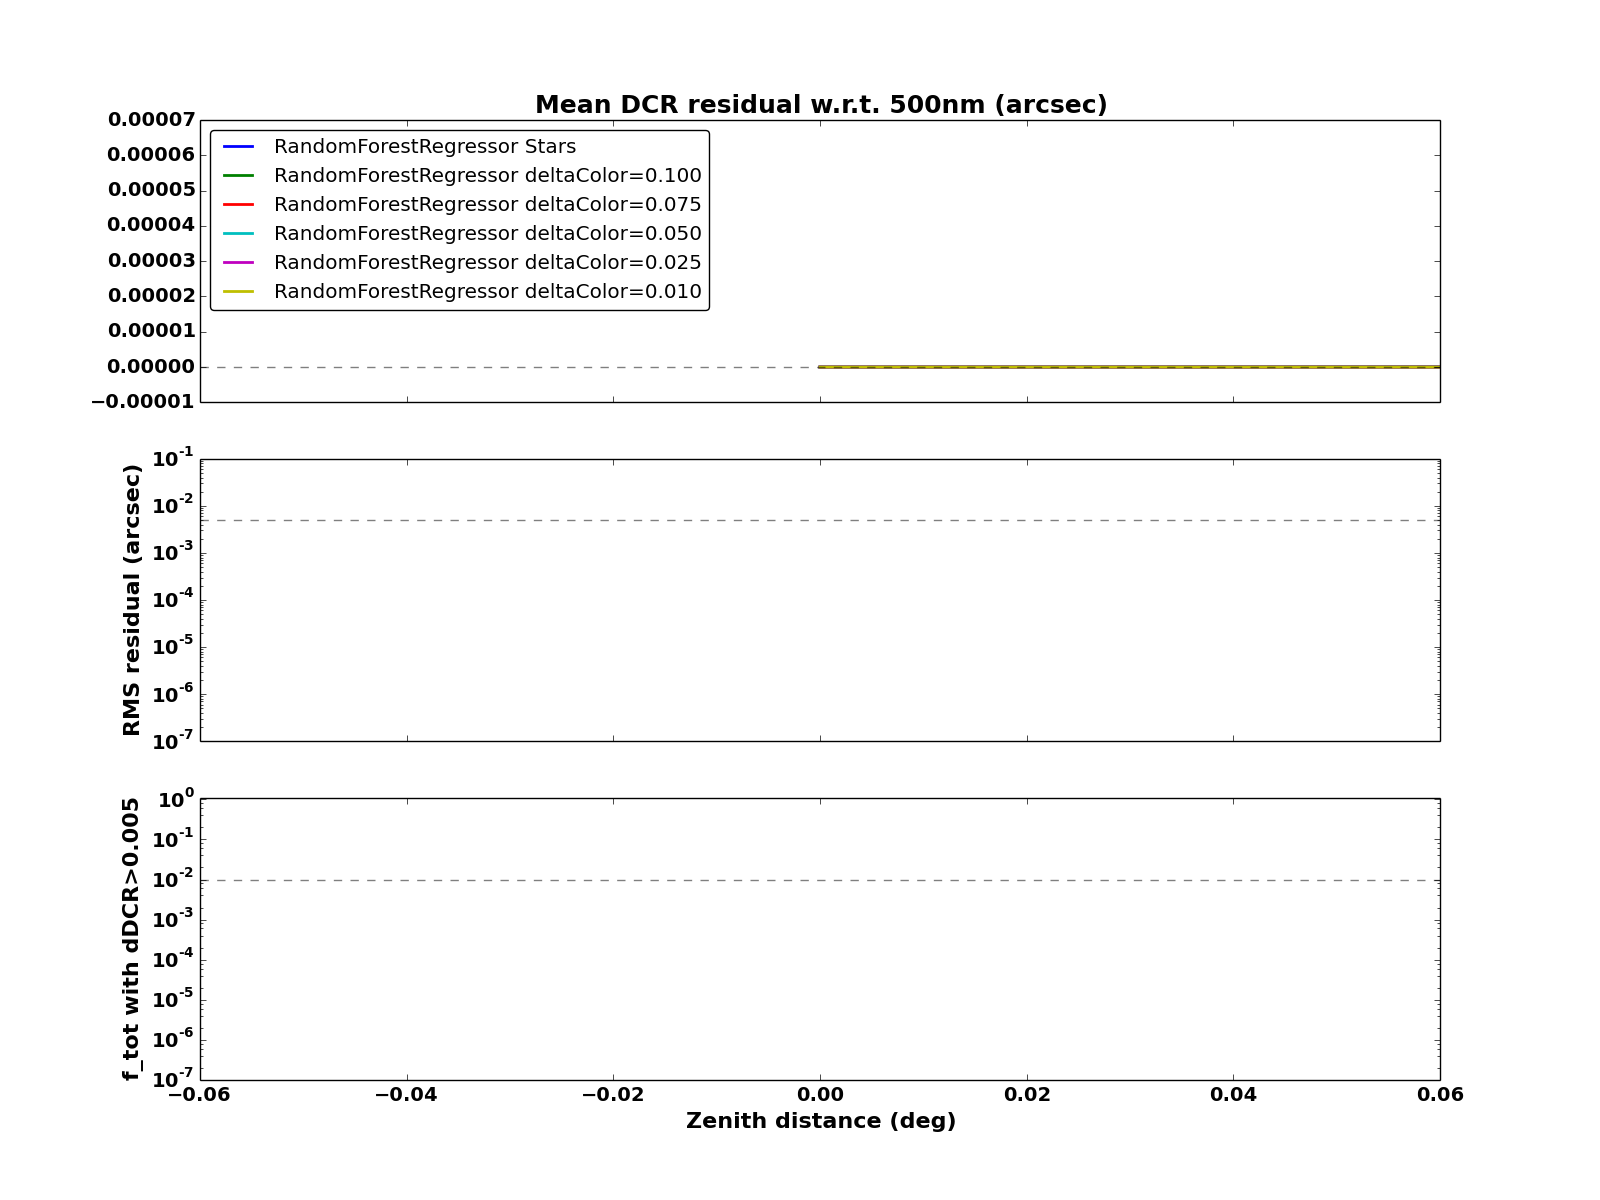
\includegraphics[width=\textwidth]{\figdir/DCR_i_deriv.png} }}
    \caption[]{{\bf Mapping Color Errors to DCR Misestimates}: (cont)}
    \label{dcrerr2}
\end{figure}
\begin{figure}
    \ContinuedFloat 
    \centering
    \subfloat[$z$--band]{{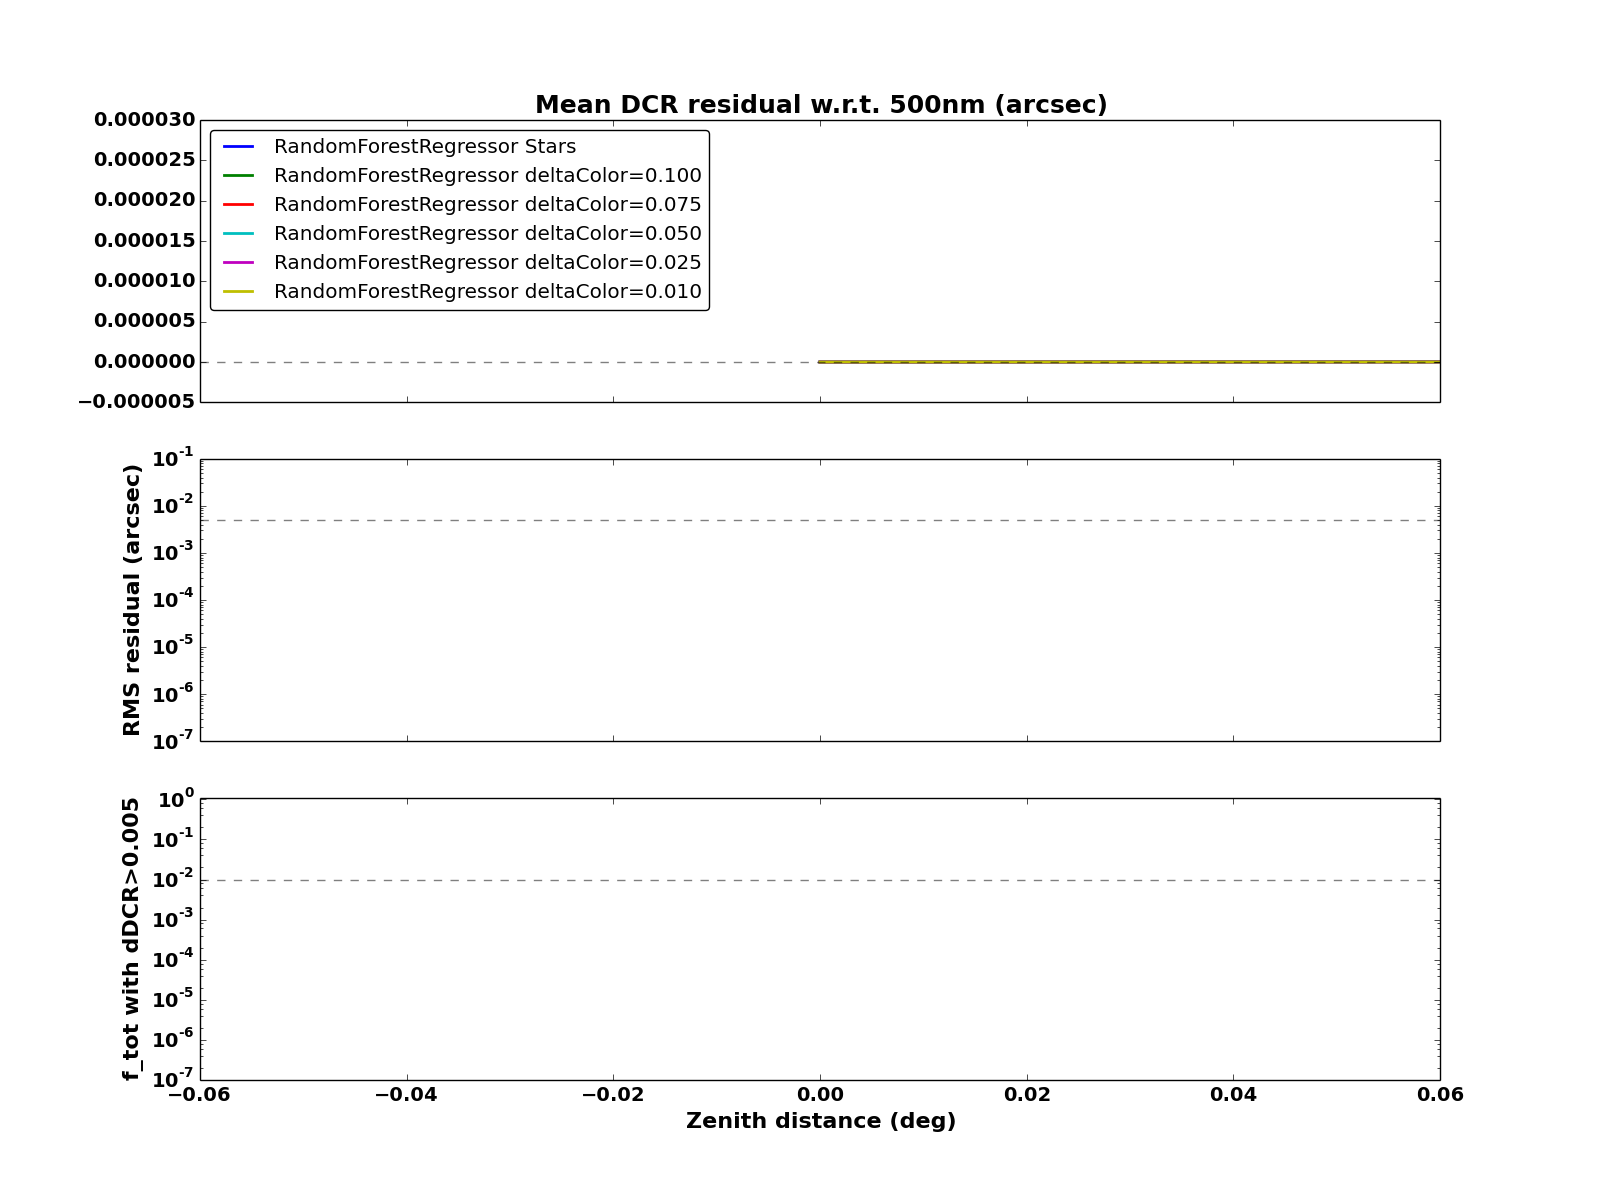
\includegraphics[width=\textwidth]{\figdir/DCR_z_deriv.png} }}
    \caption[]{{\bf Mapping Color Errors to DCR Misestimates}: (cont)}
    \label{dcrerr2}
\end{figure}

\end{appendices}

\end{document}
